%%%%%%%%%%%%%%%%%%%%%%%%%%%%%%%%%%%%%%%%%%%%%%%%%%%%%%%%%%%%
%% Chapter 3 — System Fundamentals and Problem Formulation
%% (10–15 pages)
%% Purpose: describe the physical and simulated system once,
%% define all coordinate spaces and interfaces, and formulate
%% the control objective mathematically.
%%%%%%%%%%%%%%%%%%%%%%%%%%%%%%%%%%%%%%%%%%%%%%%%%%%%%%%%%%%%
\chapter{System Fundamentals and Problem Formulation}
\label{chap:system}

Chapter~\ref{chap:fundamentals} closed with a program: learn the
hydraulic actuation of the FME~500 from identifiable data, wrap the
learned models in a structured controller, and measure robustness and
adaptation as separate effects. Before any of that can be made concrete,
the system itself has to be pinned down. This chapter describes the
manipulator and its two simulated representations exactly once, so that
every later chapter can refer back here instead of re-explaining the
plant. Sections~\ref{sec:sys:platform} and~\ref{sec:sys:kinematics}
define the mechanism, its coordinate spaces, and the mappings between
them. Section~\ref{sec:sys:actuation} fixes which signals exist, which
are commanded, and which are merely estimated.
Section~\ref{sec:sys:simscape} summarizes the high-fidelity Simscape
model that generated the historical actuator-model data, and
Section~\ref{sec:sys:isaaclab} the IsaacLab environment in which
policies are trained, adaptation data is collected, and every result in
this thesis is measured. Section~\ref{sec:sys:task} defines the primary
verge-following task and the actuator authority ceiling that constrains
it, Section~\ref{sec:sys:architecture} assembles the control
architecture and the three stacks that differ inside it, and
Sections~\ref{sec:sys:problem} and~\ref{sec:sys:evaluation-criteria}
state the control problem and the criteria against which the thesis will
judge itself.

\section{Manipulator Platform}
\label{sec:sys:platform}

The MULAG FME~500 is modeled as a serial-link manipulator with five
revolute joints. Figure~\ref{fig:sys:topology} shows the kinematic
topology. The chain starts at the base frame bolted to the Unimog's
front attachment plate (link~0), continues through the slew column
(link~1), the two boom segments (links~2 and~3), and the head carrier
(link~4), and ends in the flail mowing head (link~5). Four double-acting
hydraulic cylinders actuate the first four joints. Each cylinder closes
a triangle over its joint, so cylinder extension and joint angle are
related through the linkage geometry. The fifth joint, the rotation of
the mowing head itself, carries no cylinder of its own in the
configurations studied here: it is constrained by a swivel-link
mechanism coupled to the head carrier, and the control task treats it as
passive. Throughout the thesis the four actuated cylinders are indexed
in the fixed order introduced in Chapter~\ref{chap:models}: slew
(\emph{Drehzapfen}), boom~I (\emph{Ausleger~I}), boom~II
(\emph{Ausleger~II}), and head pivot (\emph{Messerkopf-Schwenk}).

\begin{figure}[tb]
  \centering
  \begin{subfigure}[b]{.58\linewidth}
    \centering
    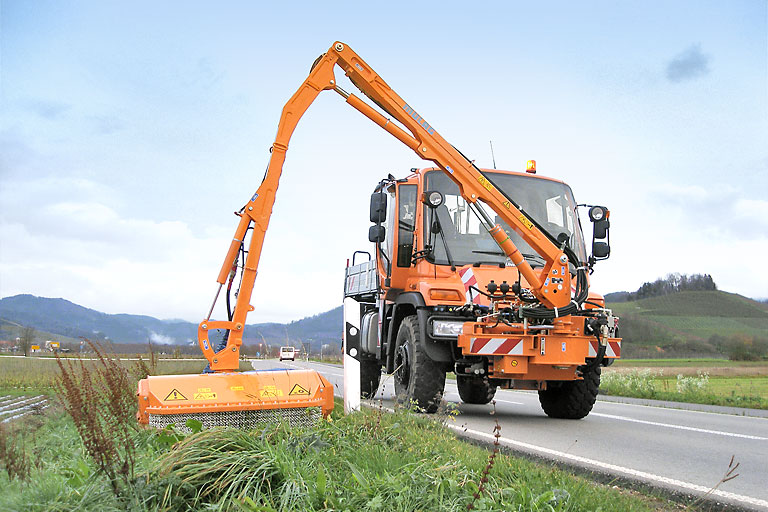
\includegraphics[width=\linewidth]{images/fme500_operation}
    \caption{}
    \label{fig:sys:fme500-photo}
  \end{subfigure}
  \hfill
  \begin{subfigure}[b]{.38\linewidth}
    \centering
    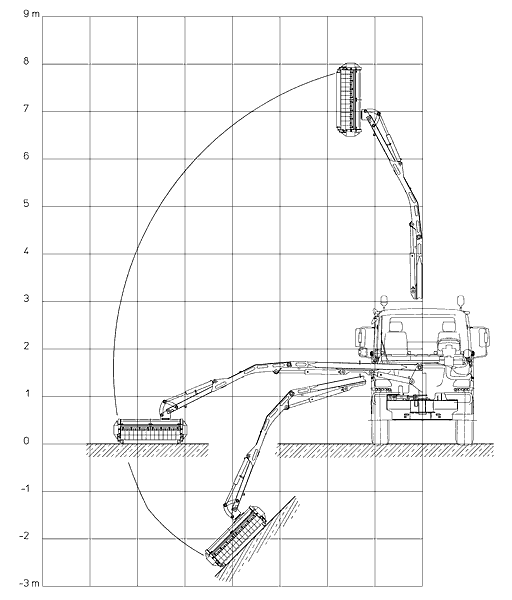
\includegraphics[width=.82\linewidth]{images/fme500_reach_diagram}
    \caption{}
    \label{fig:sys:fme500-reach}
  \end{subfigure}
  \caption{The machine studied in this thesis, as delivered. (a)~MULAG FME~500 front
  mower on a Unimog implement carrier during roadside mowing. The
  multi-link hydraulic boom holds the flail head against the verge while
  the vehicle drives. (b)~Manufacturer's working envelope of the boom,
  spanning roughly $\unit[8]{m}$ of height and reaching below road level
  for embankment mowing. Images: MULAG Fahrzeugwerk~\cite{mulag2024fme500}.}
  \label{fig:sys:fme500}
\end{figure}

\begin{figure}[tb]
  \centering
  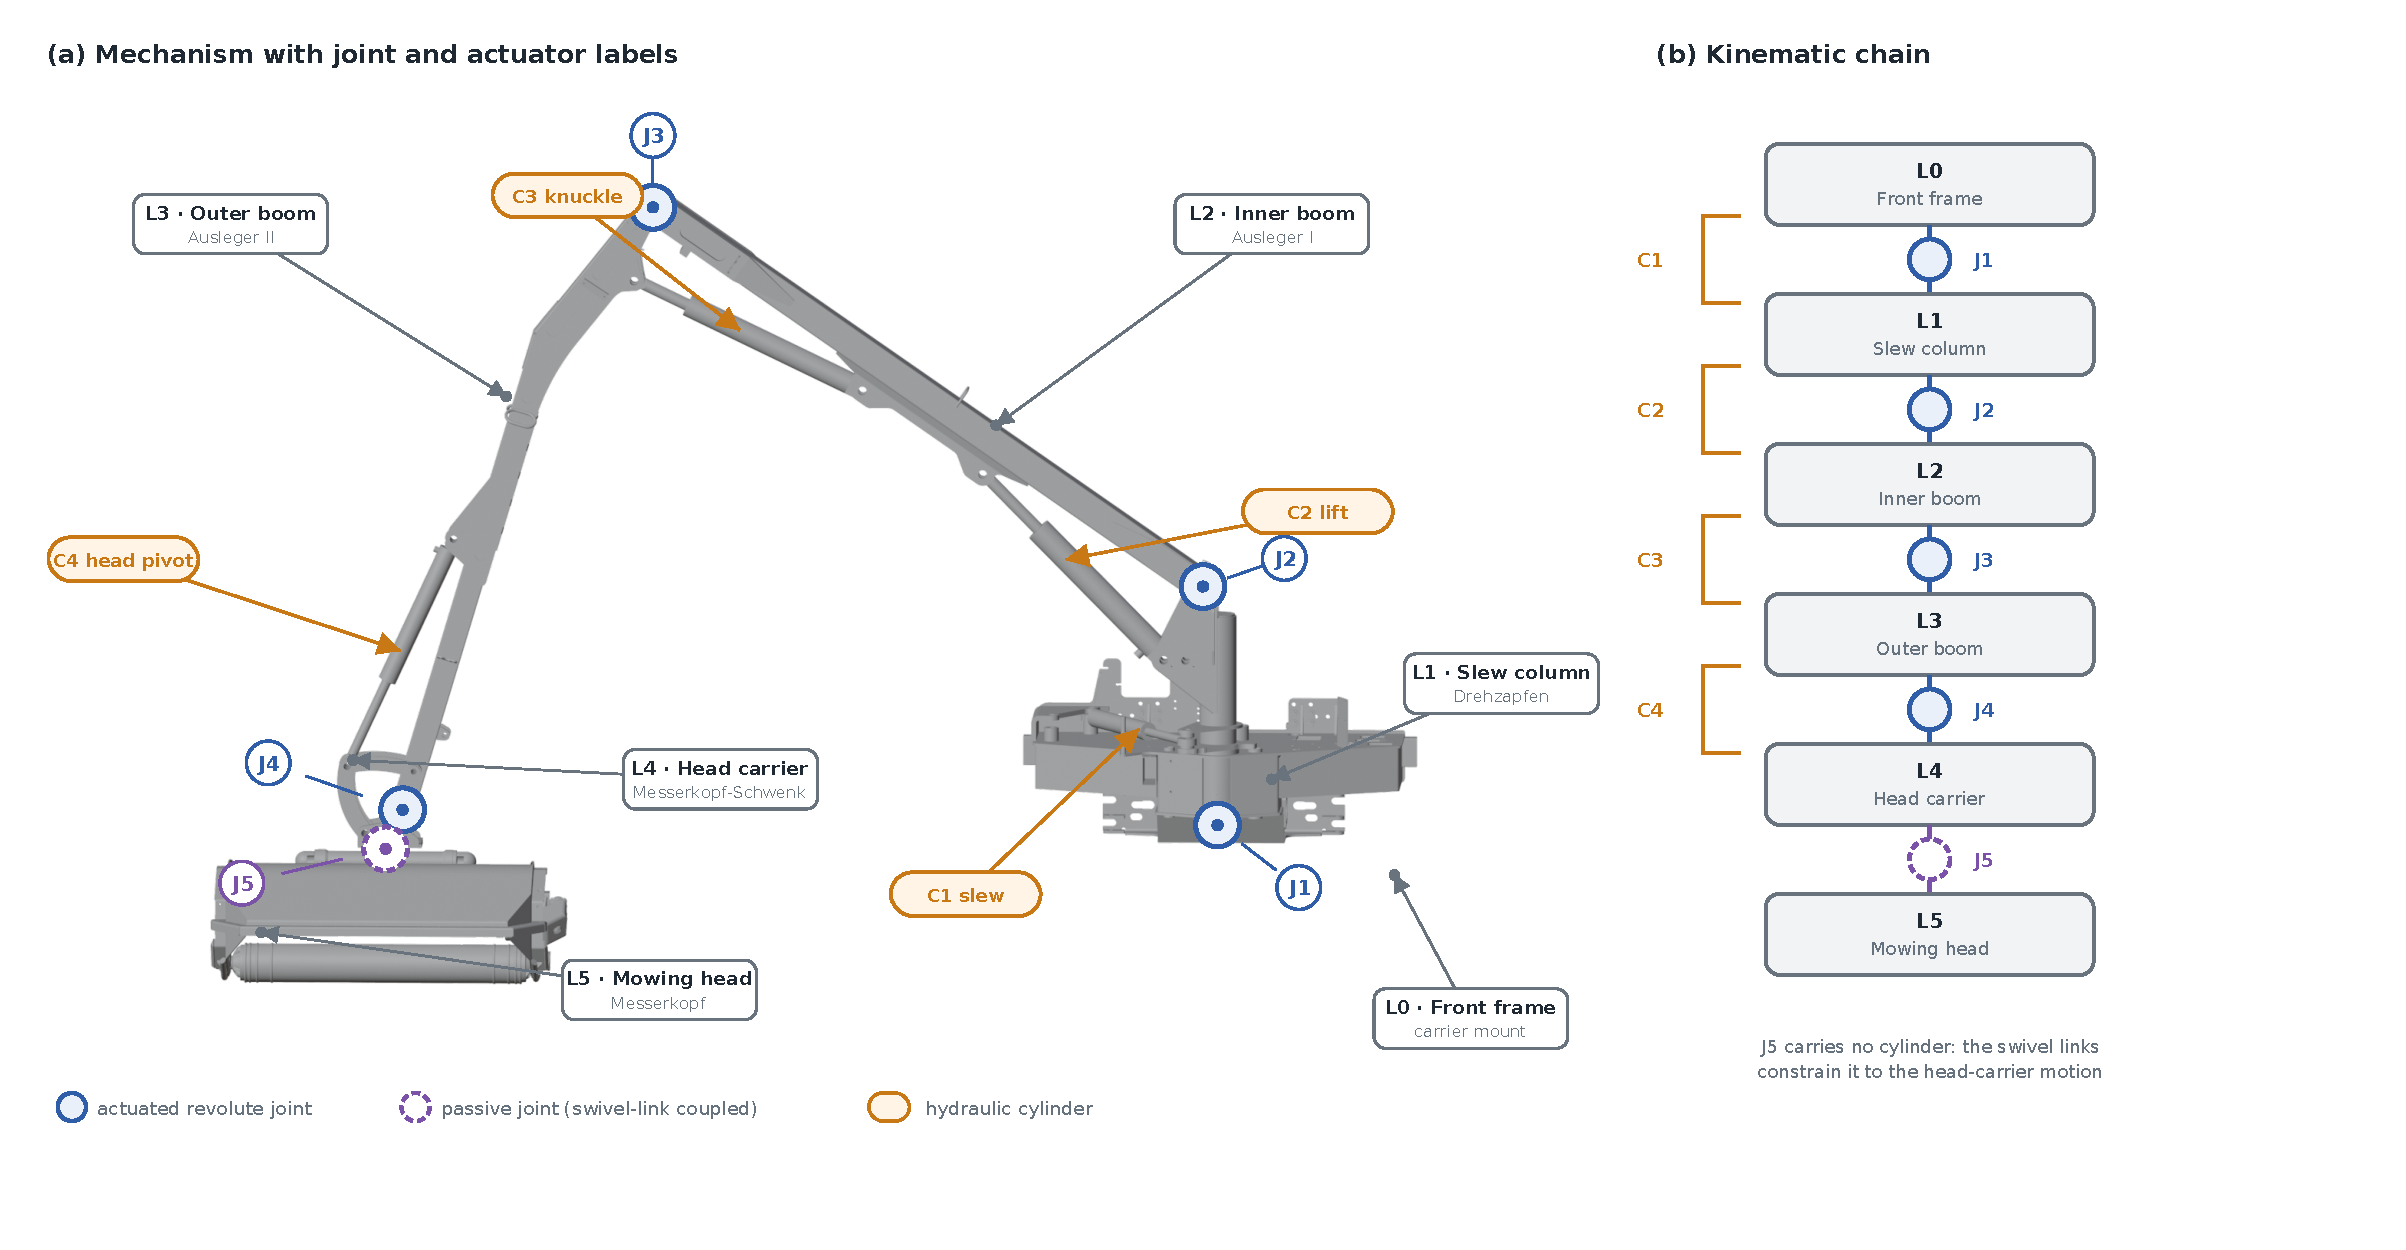
\includegraphics[width=\textwidth]{images/fme500_topology_annotated}
  \caption{Kinematic topology of the MULAG FME~500, rendered from the
  CAD model. (a)~The mechanism with every link (L0--L5), joint
  (J1--J5), and cylinder (C1--C4) called out; J5 is drawn dashed to
  mark it as passive. (b)~The same structure as an abstract chain:
  five revolute joints in series, four of them each bracketed by the
  cylinder that actuates it, and the passive fifth joint coupled
  through swivel links rather than a cylinder of its own.}
  \label{fig:sys:topology}
\end{figure}

The geometry is not hand-approximated. Link shapes, masses, centers of
mass, and full inertia tensors were extracted from the manufacturer's
CAD data using the Blender add-on
Phobos~\cite{vonszadkowski2020phobos}, which exports a consistent URDF
description of the mechanism. Figure~\ref{fig:sys:cad} renders this
CAD-derived model directly. This matters for a machine like the
FME~500: the boom is a long, asymmetric weldment whose cross-inertia
terms are significant, and a lumped-mass approximation would
misrepresent the very load coupling that makes the hydraulics hard to
control. The same CAD-derived description is the common ancestor of
both simulated representations used in this thesis, the Simscape model
of Section~\ref{sec:sys:simscape} and the IsaacLab articulation of
Section~\ref{sec:sys:isaaclab}, so their mechanical parameters agree by
construction.

Table~\ref{tab:sys:cylinders} lists the actuated joints and the
extension ranges of their cylinders as observed across the training
data. Two geometric facts recur throughout the thesis. First, the
controlled point is not the origin of the head body: the cutter contact
point sits $\unit[0.79]{m}$ below the \emph{Messerkopf} body origin,
and all task-space errors are measured at this offset tool tip. Second,
the mowing pose of interest keeps the head facing straight down. The
head-pivot cylinder holds a dedicated reference extension
($\unit[0.589]{m}$) to maintain this orientation, which effectively
reserves the fourth cylinder for the orientation task and leaves
cylinders~1--3 for positioning.

\begin{table}[tb]
  \centering
  \caption{Actuated joints of the modeled FME~500 and the extension
  ranges of their cylinders observed in the training data
  (Chapter~\ref{chap:data}).}
  \label{tab:sys:cylinders}
  \begin{tabular}{clcc}
    \toprule
    $i$ & Joint (German designation) & Function & Extension range [m] \\
    \midrule
    1 & \emph{Drehzapfen}         & slew about vertical axis & $0.018$ -- $0.493$ \\
    2 & \emph{Ausleger I}         & inner boom elevation     & $0.275$ -- $0.791$ \\
    3 & \emph{Ausleger II}        & outer boom articulation  & $0.309$ -- $0.857$ \\
    4 & \emph{Messerkopf-Schwenk} & head pivot (orientation) & $0.269$ -- $0.689$ \\
    \midrule
    5 & \emph{Messerkopf}         & head rotation, passive (swivel links) & --- \\
    \bottomrule
  \end{tabular}
\end{table}

\begin{figure}[tb]
  \centering
  \begin{subfigure}[b]{.47\linewidth}
    \centering
    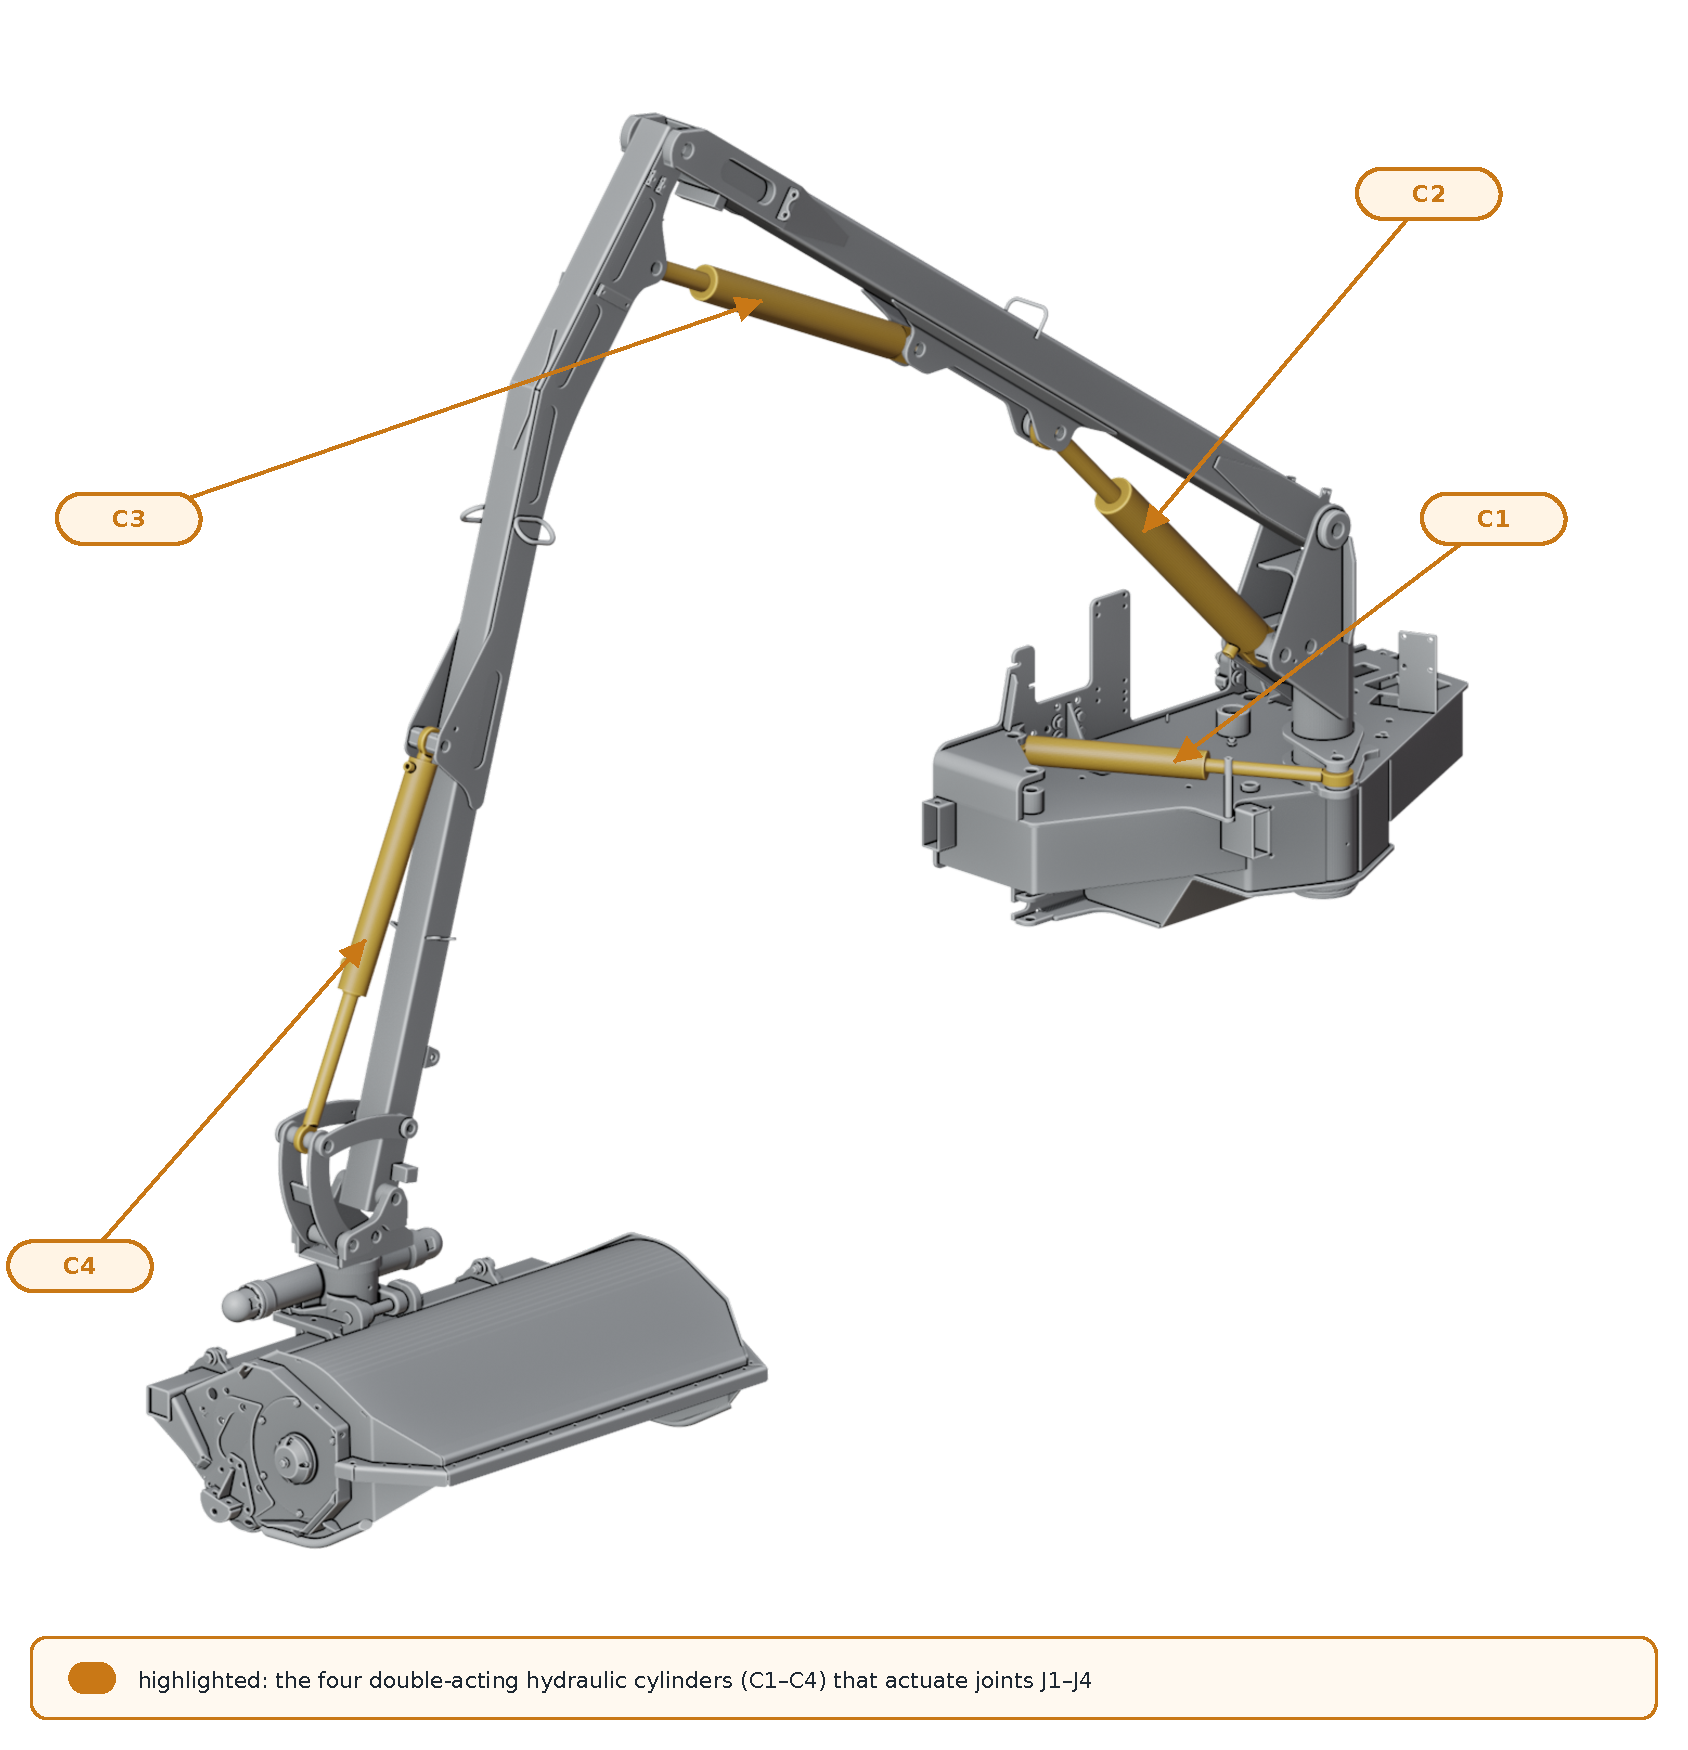
\includegraphics[width=\linewidth]{images/fme500_cad_iso_annot}
    \caption{}
    \label{fig:sys:cad-iso}
  \end{subfigure}
  \hfill
  \begin{subfigure}[b]{.49\linewidth}
    \centering
    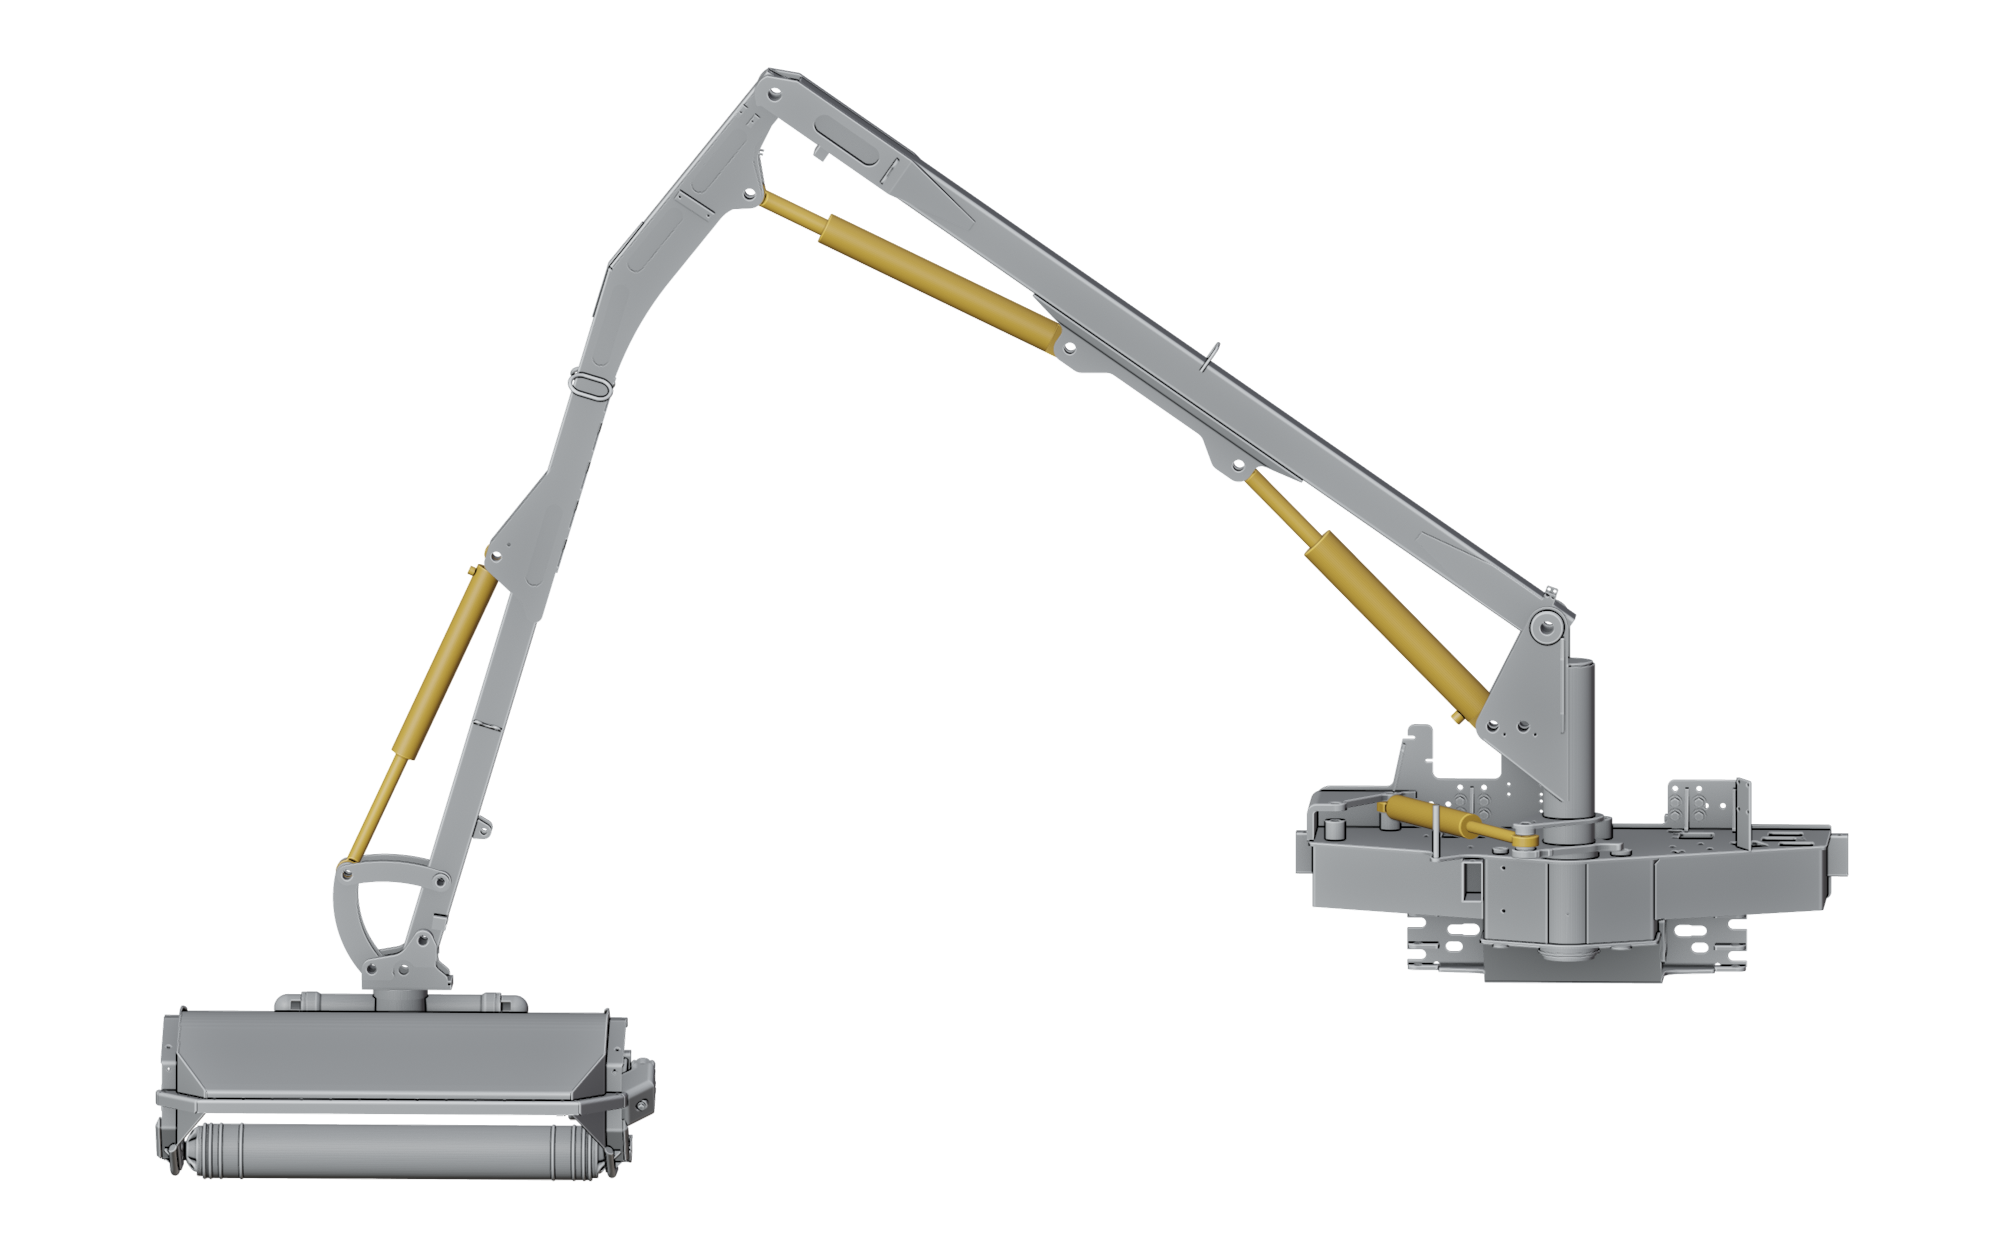
\includegraphics[width=\linewidth]{images/fme500_cad_side}
    \caption{}
    \label{fig:sys:cad-side}
  \end{subfigure}
  \caption{The CAD-derived multibody model of the FME~500 arm, rendered
  from the URDF export used throughout this thesis: (a)~isometric view
  with the four hydraulic cylinders C1--C4 highlighted in orange and
  labeled, (b)~side elevation in the folded zero pose. The swivel links
  of the passive fifth joint connect the head carrier to the flail
  head, and the base frame carries the slew column. The same geometry,
  masses, and inertia tensors drive both the Simscape multibody model
  and the IsaacLab articulation.}
  \label{fig:sys:cad}
\end{figure}

To make the serial chain concrete, Figure~\ref{fig:sys:links} shows the
individual rigid bodies as they are imported from the URDF, each
rendered on its own in an orthographic view. Reading outward from the
vehicle: the \emph{front frame} (link~0) bolts to the Unimog attachment
plate and carries the slew bearing; the \emph{slew column}
(\emph{Drehzapfen}, link~1) rotates the whole arm about the vertical
axis; the \emph{inner} and \emph{outer boom} segments
(\emph{Ausleger~I} and~\emph{II}, links~2 and~3) are the long
load-bearing weldments whose asymmetric cross-sections give the
significant cross-inertia terms noted above; the \emph{head carrier}
(\emph{Messerkopf-Schwenk}, link~4) with its swivel-link pair sets the
head orientation; and the \emph{flail mowing head} (link~5) does the
cutting. The final card in Figure~\ref{fig:sys:links} shows one of the four
double-acting cylinders as a separate barrel--rod pair, the form in
which each actuator enters the closed kinematic loop of
Section~\ref{sec:sys:kinematics}.

\begin{figure}[tb]
  \centering
  \newcommand{\linkcell}[3]{%
    \begin{subfigure}[b]{#1\linewidth}
      \centering
      \includegraphics[height=32mm]{images/links/link_#2}
      \caption{#3}
    \end{subfigure}}
  \linkcell{.31}{frontrahmen}{Front frame (link 0)}\hfill
  \linkcell{.31}{drehzapfen}{Slew column (link 1)}\hfill
  \linkcell{.31}{ausleger_i}{Inner boom (link 2)}

  \vspace{3mm}
  \linkcell{.31}{ausleger_ii}{Outer boom (link 3)}\hfill
  \linkcell{.31}{messerkopf_schwenk}{Head carrier (link 4)}\hfill
  \linkcell{.31}{messerkopf}{Mowing head (link 5)}

  \vspace{3mm}
  \begin{subfigure}[b]{.31\linewidth}
    \centering
    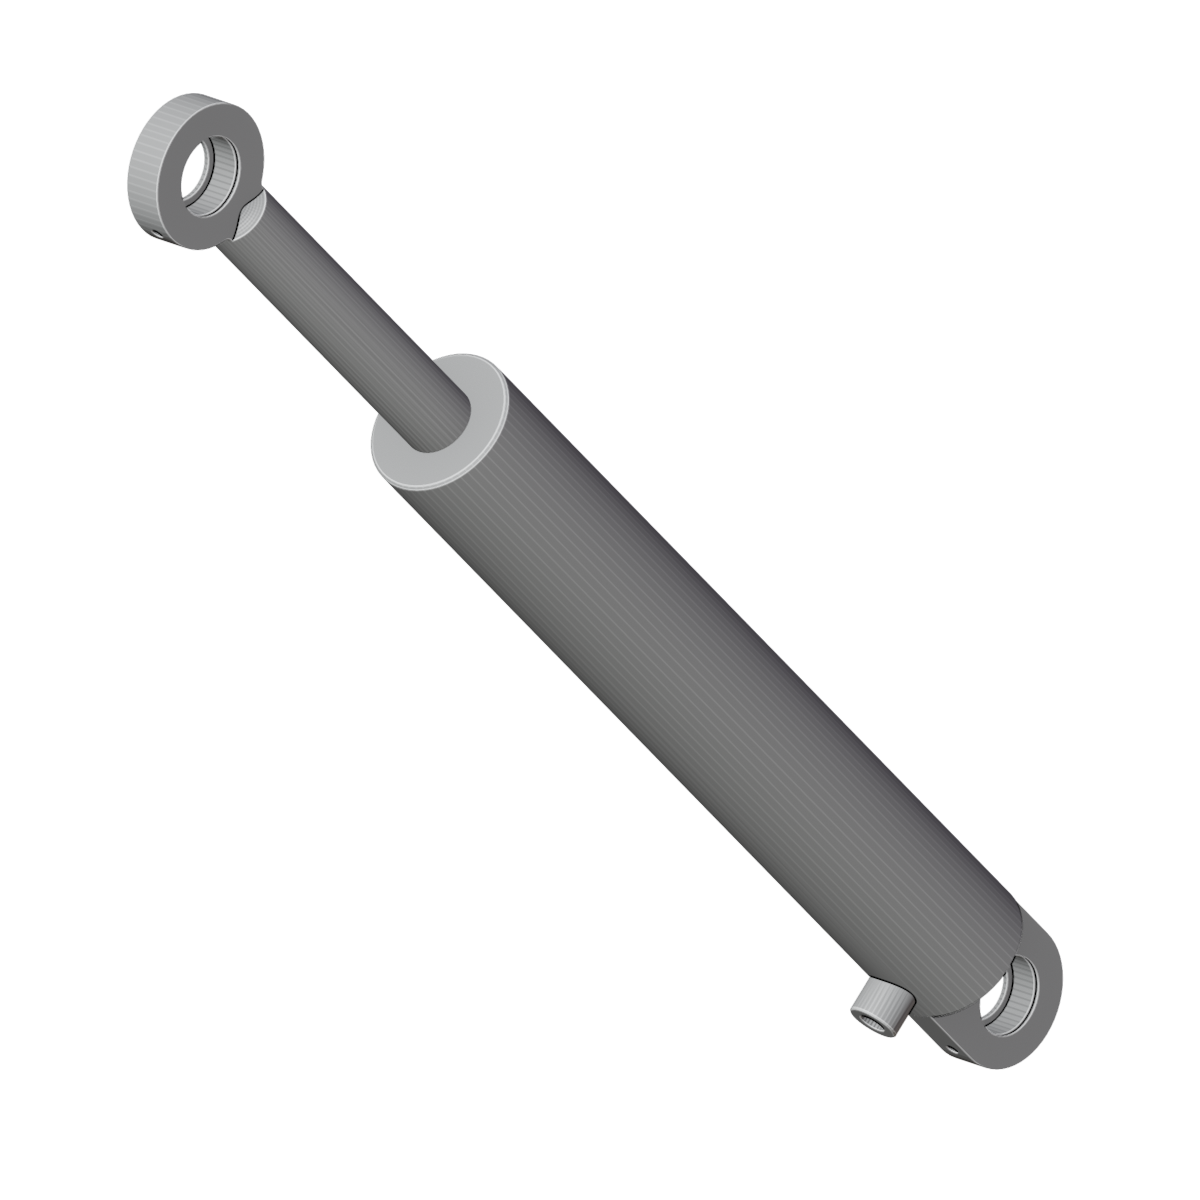
\includegraphics[height=32mm]{images/links/link_cylinder}
    \caption{Cylinder (barrel + rod)}
  \end{subfigure}
  \caption{Catalog of the FME~500 rigid bodies, each rendered
  individually from the URDF geometry in an orthographic view. Links 0--5
  form the serial chain; (g)~shows one of the four hydraulic cylinders as
  the barrel--rod pair that actuates a joint. Renders share the coordinate
  frames, scale, and matte engineering style used throughout the thesis.}
  \label{fig:sys:links}
\end{figure}

\section{Kinematic Structure and Coordinate Mappings}
\label{sec:sys:kinematics}

\subsection{Joint Space and Cylinder Space}

The mechanism's configuration is described by the joint vector
$\bm{q} \in \mathbb{R}^5$ and its velocity $\dot{\bm{q}}$. The actuated
coordinates, however, are the cylinder extensions
$\bm{x} \in \mathbb{R}^4$ introduced in Chapter~\ref{chap:models}. Each
cylinder connects an attachment point $\bm{p}_A$ on link $k$ to a point
$\bm{p}_B$ on link $k{+}1$, both fixed in their links and exported from
the CAD data. The instantaneous cylinder length and extension are
%
\begin{equation}
  \label{eq:sys:cyl-length}
  \ell_i(\bm{q}) = \bigl\| \bm{p}_B(\bm{q}) - \bm{p}_A(\bm{q}) \bigr\|,
  \qquad
  x_i = \ell_i(\bm{q}) - \ell_{0,i},
\end{equation}
%
with $\ell_{0,i}$ the retracted reference length. Differentiating
\eqref{eq:sys:cyl-length} gives the scalar mapping between joint motion
and extension rate,
%
\begin{equation}
  \label{eq:sys:cyl-jac}
  \dot{x}_i = J_{\mathrm{cyl},i}(\bm{q})\, \dot{\bm{q}},
  \qquad
  J_{\mathrm{cyl},i} = \bm{e}_i^{\!\top}
  \bigl( \bm{J}_B - \bm{J}_A \bigr),
\end{equation}
%
where $\bm{e}_i$ is the unit vector along the cylinder axis and
$\bm{J}_A, \bm{J}_B$ are the translational Jacobians of the attachment
points. The same mapping carries force back to torque: by the principle
of virtual work, a cylinder force $F_{h,i}$ contributes the joint
torque $\bm{\tau}_{\mathrm{act}} = \bm{J}_{\mathrm{cyl}}^{\top}
\bm{F}_h$. The rows of $\bm{J}_{\mathrm{cyl}}$ are the lever arms
discussed qualitatively in Chapter~\ref{chap:fundamentals}. They vary
over the stroke, and with them the effective gain and stiffness that
each cylinder presents to its joint.

\subsection{Task Space and the Calibrated Cutter Jacobian}
\label{sec:sys:task-jacobian}

The task is defined at the cutter tip, expressed in the truck chassis
frame (\texttt{base\_link}). This choice is deliberate and matters in
practice: the articulation root of the simulated arm is the slew base,
which moves with the arm, and using it as the reference frame corrupts
every tracking measurement. All references and errors in this thesis
live in the truck frame, and the controlled point includes the
$\unit[-0.79]{m}$ tool-tip offset of Section~\ref{sec:sys:platform}.
Because the truck itself drives forward during the primary task
(Section~\ref{sec:sys:task}), the chassis frame translates along the
road while the errors are measured inside it. The along-track direction
is supplied by the vehicle and is not a controlled degree of freedom.

For control, the composition of task kinematics and cylinder linkage is
captured in a single calibrated Jacobian
$\bm{J}_c \in \mathbb{R}^{3\times4}$ that maps cylinder extension rates
to cutter-tip velocity in the truck frame. Rather than deriving it
symbolically through the CAD chain, it was measured directly on the
simulated plant: starting from the head-down mowing configuration, each
cylinder target was stepped in turn and the settled cutter displacement
recorded, giving central-difference estimates of every column. The
measured matrix has rank~3 with singular values $8.24$, $5.69$, and
$2.79$, confirming that at the mowing operating point the four
cylinders span exactly three independent task directions. This is the
quantitative form of the observation from
Section~\ref{sec:sys:platform}: with cylinder~4 committed to holding
the head down, the remaining freedom moves the cutter in a
three-dimensional workspace, and one direction of the nominal base
frame is reachable only through vehicle motion. The damped
least-squares controller of Chapter~\ref{chap:control} inverts this measured $\bm{J}_c$, so the nominal layer and the plant share one
geometric contract.

\section{Actuation and Measured State}
\label{sec:sys:actuation}

Every interface in this thesis draws from one signal inventory, and it is stated once here, together with who can see what.
Table~\ref{tab:sys:signals} summarizes the quantities, their
dimensions, and their availability in the two simulation environments.

\begin{table}[tb]
  \centering
  \caption{Signal inventory of the modeled system. ``S'' marks signals
  present in the Simscape data exports, ``I'' signals available live in
  the IsaacLab environment, ``M'' quantities that exist there only
  through the learned models of Chapter~\ref{chap:models}, and ``P''
  \emph{privileged} quantities that exist in simulation but must never
  enter a deployable policy or estimator input.}
  \label{tab:sys:signals}
  \small
  \begin{tabular}{llcl}
    \toprule
    Signal & Dimension & Availability & Meaning \\
    \midrule
    $\bm{u}$ & $[-1,1]^4$ & S, M & normalized proportional-valve commands \\
    $\bm{x},\, \dot{\bm{x}}$ & $\mathbb{R}^4$ & S, I & cylinder extensions and velocities \\
    $\Delta\bm{p}$ & $\mathbb{R}^4$ & S, M & chamber pressure differences \\
    $\bm{F}$ & $\mathbb{R}^4$ & S & logged rod forces \\
    $\bm{q},\, \dot{\bm{q}}$ & $\mathbb{R}^5$ & S, I & joint positions and velocities \\
    $\bm{p}_c$ & $\mathbb{R}^3$ & S, I & cutter-tip position, truck frame \\
    $\bm{h}$ & $\mathbb{R}^{9}$ & I & forward terrain-height profile ahead of the cutter \\
    $\bm{c} = [\Delta\bm{x}^*, \Delta\dot{\bm{x}}^*]$ & $\mathbb{R}^8$ & I & desired cylinder command \\
    $\factorvec$ & $\mathbb{R}^6$ & P & physical randomization factors of the active plant \\
    $\bm{z} = \mu(\factorvec)$ & $\mathbb{R}^{d_z}$ & P & privileged dynamics latent, $d_z = 2$ \\
    $\latenthat$ & $\mathbb{R}^{d_z}$ & M & AAM estimate of $\bm{z}$ from observable history \\
    \bottomrule
  \end{tabular}
\end{table}

The separation encoded in that table drives several design decisions.
The valve command $\bm{u}$ exists only inside the Simscape plant and
its data exports. In IsaacLab no valve is simulated, so any model that
needs valve information at runtime must either receive it from a
learned inverse model (the \ppoIDFD{} and \ppoIDAAMFD{} paths) or
predict it internally (the reduced-order model of the \ppoROM{} path).
The pressure difference $\Delta\bm{p}$ likewise has no native
counterpart in the rigid-body simulation. At runtime it is a recursive
internal state of the learned actuator models rather than a
measurement, and it is deliberately withheld from the deployment-mirror
inputs of Chapter~\ref{chap:models} so that the causal history estimator
cannot lean on a quantity a real machine would not publish. Only
positions and velocities, of cylinders, joints, and the cutter tip,
together with the terrain scan, are common ground, which is why the
acceptance gates of Section~\ref{sec:sys:evaluation-criteria} are formulated on these quantities.

The last three rows carry the rule that governs the whole adaptation
argument. The factor vector $\factorvec$ and the latent
$\bm{z} = \mu(\factorvec)$ derived from it are privileged: they are
known to the simulator, they are used to \emph{train} and to
\emph{audit}, and they are never read by anything that claims to be
deployable. Only $\latenthat$, inferred from causal observable history,
may enter the adaptive stack. Commanded quantities carry a star and
estimated ones a hat, following the notation of
Chapter~\ref{chap:models}; $\latenthat$ exists only in \ppoIDAAMFD.

\section{High-Fidelity Simscape Model}
\label{sec:sys:simscape}

The primary data source for the \emph{actuator} models of this thesis
(the command-conditioned reduced-order model and the inverse/forward
pair) is a multi-domain Simscape model of the FME~500 that I
developed in the master project preceding this thesis. This section
summarizes the parts of that model the thesis depends on. The modeling
and validation work itself is part of the contribution of this research
program.

The division of provenance is stated explicitly, because the data campaigns
of Chapter~\ref{chap:data} are easy to conflate and the three actuator
paths do \emph{not} share the same one.
Table~\ref{tab:sys:provenance} states it once.

\begin{table}[tb]
  \centering
  \caption{Provenance of each frozen actuator component. The command ROM
  is the only one that has been calibrated against the deployment plant;
  the inverse/forward pair is Simscape-identified throughout. This
  asymmetry is a property of the comparison and is carried into the
  discussion of Chapter~\ref{chap:evaluation}, not glossed over.}
  \label{tab:sys:provenance}
  \small
  \begin{tabular}{lp{4.4cm}p{5.0cm}}
    \toprule
    Component & Identified on & Calibrated on \\
    \midrule
    Command ROM & Simscape closed-loop export (grey-box, full model)
      & IsaacLab/PhysX closed-loop rollouts, via a bounded command-gated
        correction head only \\
    Control ID & Simscape closed-loop export & --- \\
    Strict FD & Simscape closed-loop export, retrained on the strict
        open-loop excitation export & --- \\
    $SD_0$, $\mu(\factorvec)$, $SD_z$, AAM
      & IsaacLab/PhysX adaptation collection (from scratch) & --- \\
    \bottomrule
  \end{tabular}
\end{table}

The Simscape model is therefore \emph{historical} provenance for the
bulk of every actuator model, and the sole provenance of the frozen ID
and strict FD checkpoints, which are carried forward unchanged. It is
not the whole story for the command ROM: after its Simscape training the
ROM received a small, bounded, closed-loop calibration inside IsaacLab
itself, described in Section~\ref{sec:models:rom-calibration}. And it
produced nothing at all for the adaptation chain: the system-dynamics
surrogate, the privileged factor encoder, and the AAM are trained from
scratch on data collected in IsaacLab through the command ROM and PhysX
(Section~\ref{sec:sys:isaaclab}).

\subsection{The Command ROM as Deployment Actuator}
\label{sec:sys:rom-is-plant}

The reason the ROM alone was calibrated against PhysX, and the reason
the adaptation data was collected through it, is a single design
decision that has to be stated explicitly because everything downstream
depends on it: \emph{the command ROM plus PhysX is the deployment plant
of this thesis}. Inside the simulator it stands in for the real
hydraulic machine. The Simscape model is too slow to be that stand-in
(Section~\ref{sec:fund:sim-data-source}) and the bare PhysX articulation
has no hydraulics at all, so the hydraulically structured, PhysX-calibrated
ROM is the best available representation of the machine that can run at
policy-training throughput. That is why it is the model that was allowed
to see the deployment loop, and why the system-dynamics surrogate and
the AAM describe \emph{it} rather than Simscape.

This gives the ROM two roles at once, and the thesis must not let them
blur. It is the plant, and it is also the actuator of \ppoROM. The
consequence for the three-way comparison is direct and is carried into
Chapter~\ref{chap:evaluation} rather than left implicit:

\begin{itemize}
  \item \ppoROM{} is the stack whose actuator \emph{coincides with the
    plant}. It therefore measures how well the task can be done when the
    actuator model is, by construction, exactly right. It is the
    reference condition, not merely the best of three models.
  \item \ppoIDFD{} substitutes an independently identified learned
    actuator pair for that plant model. It measures the cost of that substitution: what is lost when the actuator representation is
    identified elsewhere and must reproduce the deployment plant rather
    than be it.
  \item \ppoIDAAMFD{} measures how much of that cost online adaptation
    recovers.
\end{itemize}

Read this way, the comparison is well posed, and the ID transfer gap
reported in Chapter~\ref{chap:evaluation} is an expected quantity to be
measured rather than an anomaly to be explained away. Read carelessly,
\ppoROM's advantage looks like evidence that a reduced-order model is a
better function approximator than an inverse--forward pair, which is
\emph{not} what the experiment can show. Wherever \ppoROM{} is quoted as
the certified baseline in this thesis, this qualification applies.

\subsection{Mechanical Subsystem}

The mechanism is simulated as a rigid multibody system in Simscape
Multibody~\cite{mathworks2024simscape}, with the CAD-derived links,
joints, and cylinder attachment frames of
Section~\ref{sec:sys:platform}. The joint-space dynamics take the
standard manipulator form
%
\begin{equation}
  \label{eq:sys:eom}
  \bm{M}(\bm{q})\ddot{\bm{q}}
  + \bm{C}(\bm{q},\dot{\bm{q}})\dot{\bm{q}}
  + \bm{g}(\bm{q})
  + \bm{\tau}_{\mathrm{fric}}(\dot{\bm{q}})
  = \bm{\tau}_{\mathrm{act}} - \bm{J}^{\top}(\bm{q})\,\bm{F}_{\mathrm{ext}},
\end{equation}
%
with the inertia matrix $\bm{M}$ assembled from the imported CAD
tensors. Two terms deserve comment. The friction torque
$\bm{\tau}_{\mathrm{fric}}$ combines viscous and Coulomb components
with a smooth $\tanh$ approximation of the sign function, extended by a
Stribeck term at the cylinder level to capture stick--slip at low
velocities. The slew joint, which carries high side loads, is
particularly sensitive to this. The external wrench
$\bm{F}_{\mathrm{ext}}$ models the vegetation cutting load as a nominal
force plus a disturbance that scales with feed velocity and vegetation
density, rather than as a constant, so mowing does not reduce to a
static payload. Each cylinder is built as a closed kinematic loop
(spherical--prismatic--cylindrical, shown in the top band of
Figure~\ref{fig:sys:actuator-channel}), which lets it self-align under
load without over-constraining the mechanism, and hard-stop constraints
enforce the physical stroke limits of
Table~\ref{tab:sys:cylinders}.

\subsection{Hydraulic Subsystem}

\begin{figure}[tb]
  \centering
  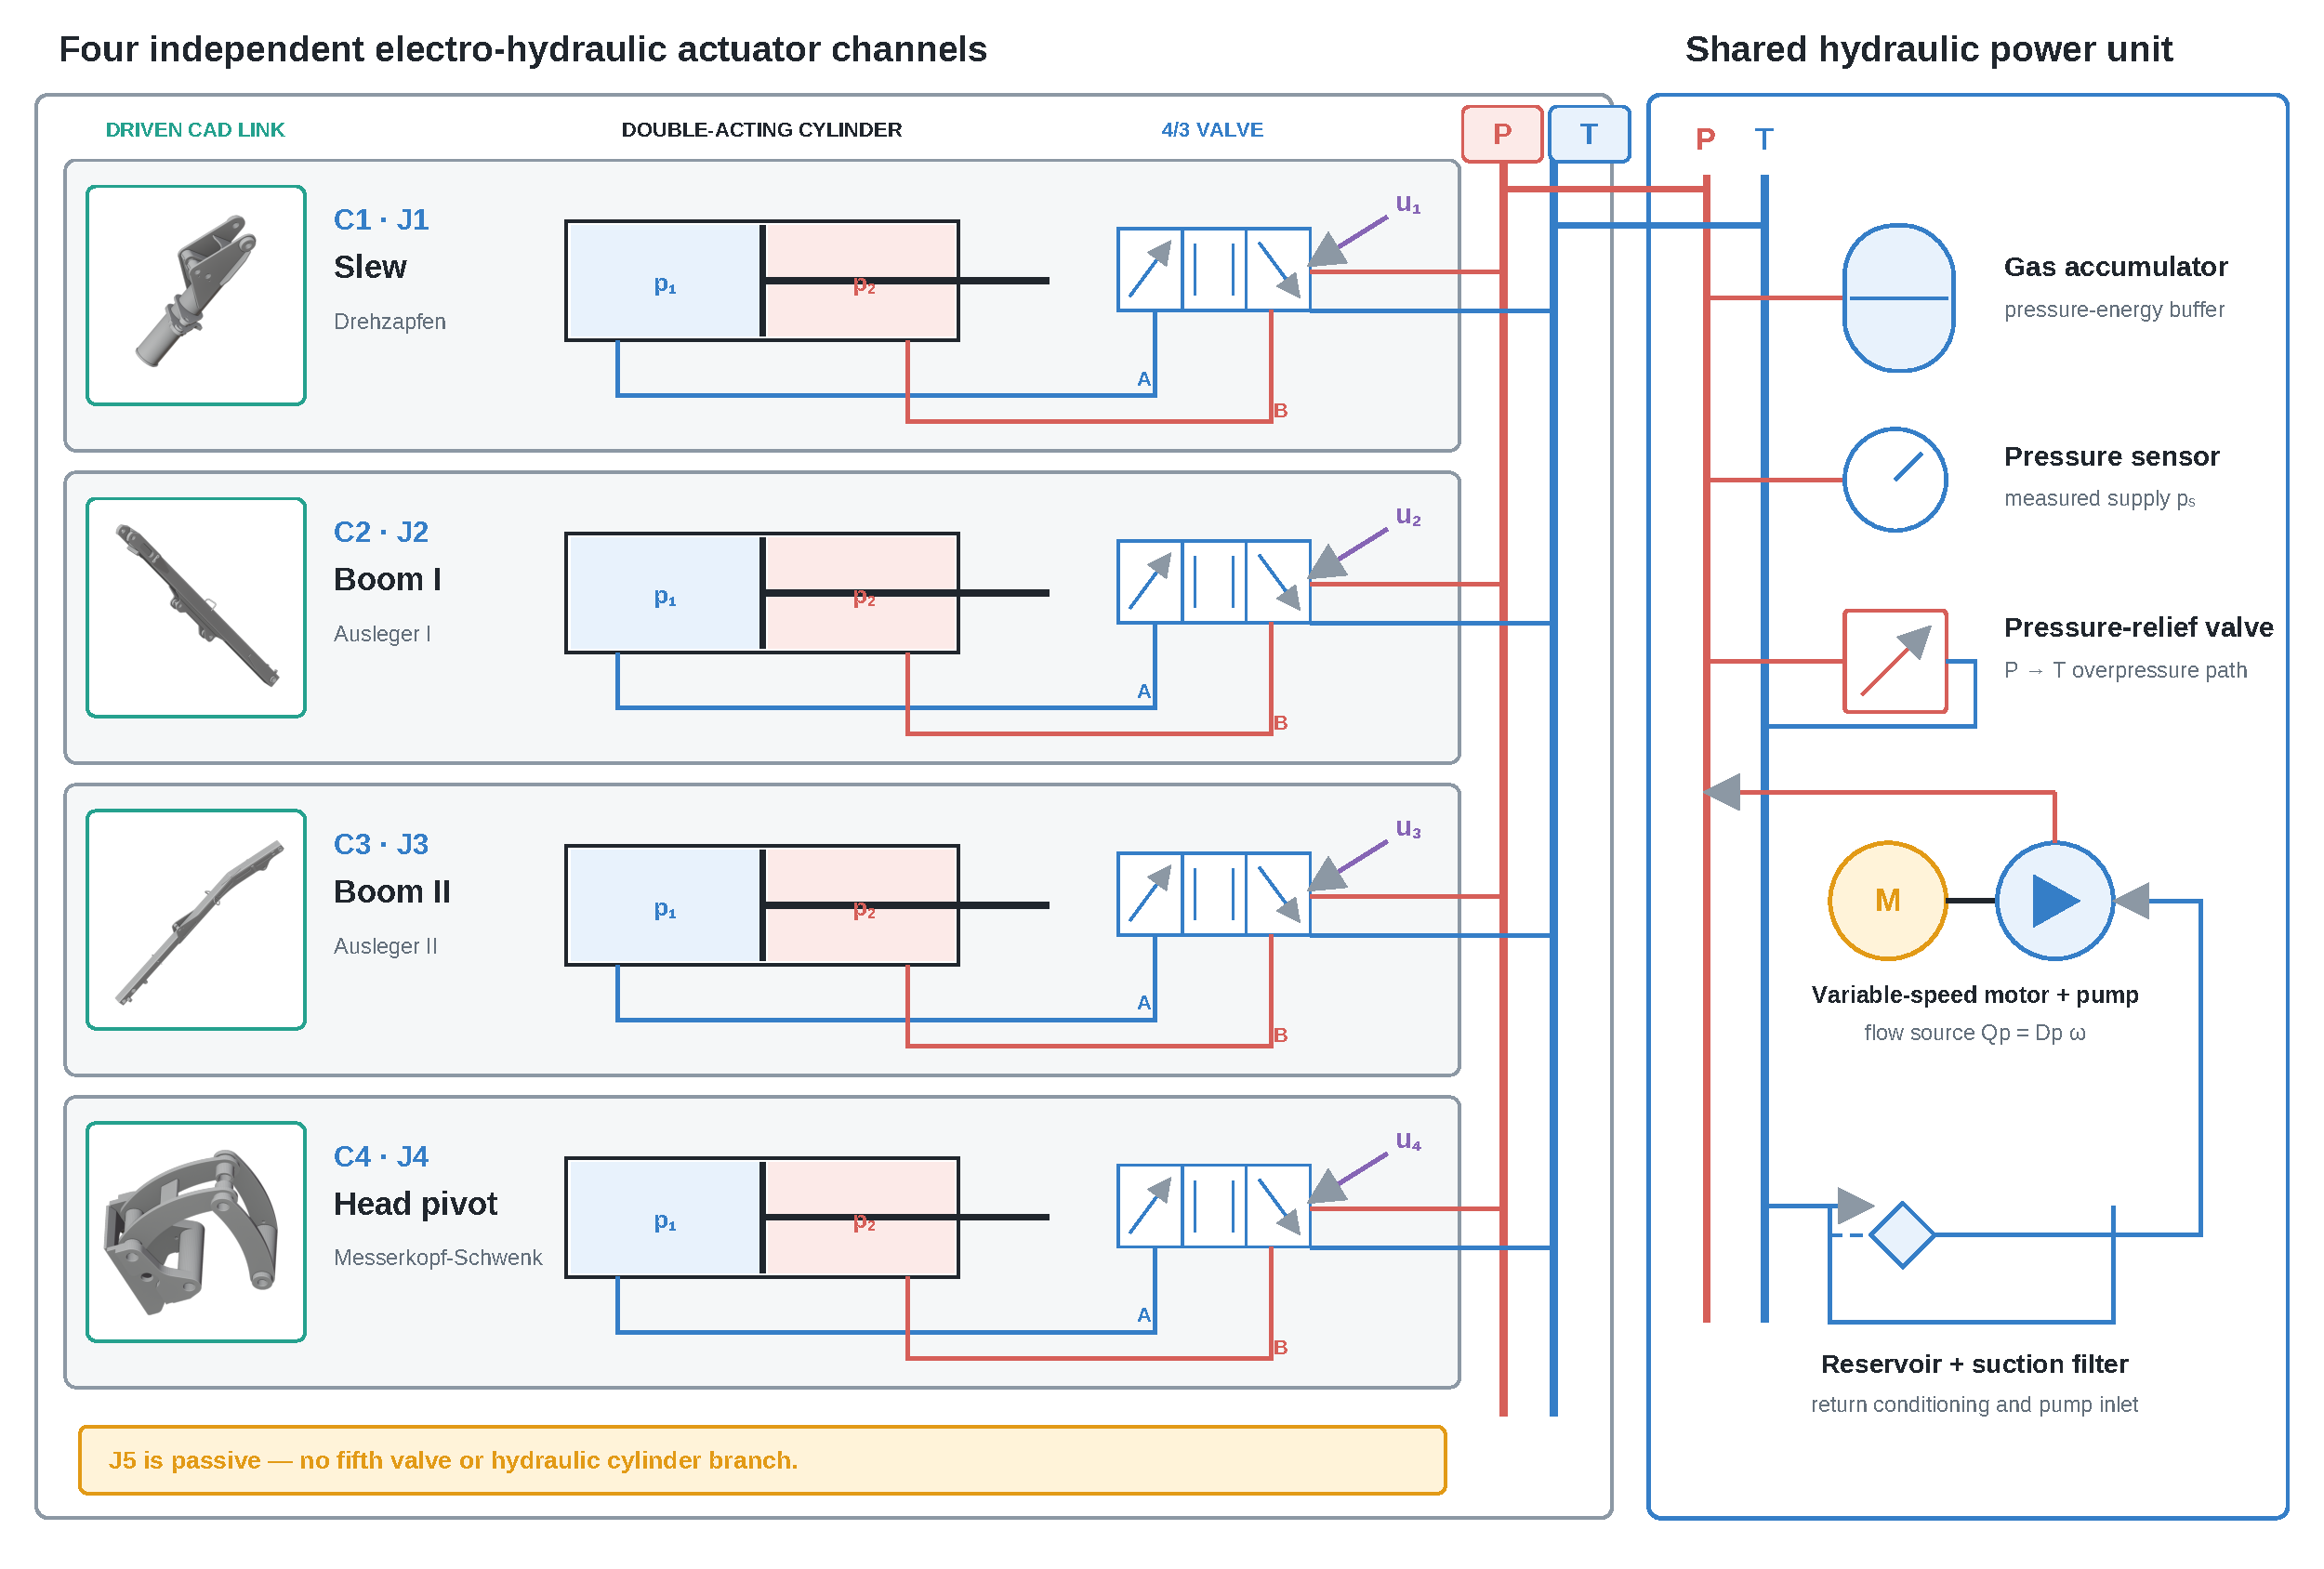
\includegraphics[width=\textwidth]{images/fme500_hydraulic_schematic}
  \caption{System-level hydraulic schematic of the modeled machine.
  Left: the four independent electro-hydraulic actuator channels, each
  a 4/3 proportional directional valve driving one double-acting
  cylinder that moves its link (thumbnails rendered from the same CAD
  model as Figures~\ref{fig:sys:topology}--\ref{fig:sys:links}). Right:
  the shared hydraulic power unit, comprising the variable-speed pump
  and its prime mover, the gas-charged accumulator, the pressure-relief
  valve, the pressure sensor, the suction filter, and the reservoir,
  connected to every channel through the common supply~(P) and
  return~(T) rails. Only four cylinders are present: the fifth joint is
  passive (Table~\ref{tab:sys:cylinders}) and carries no actuator of
  its own.}
  \label{fig:sys:schematic}
\end{figure}

\begin{figure}[tb]
  \centering
  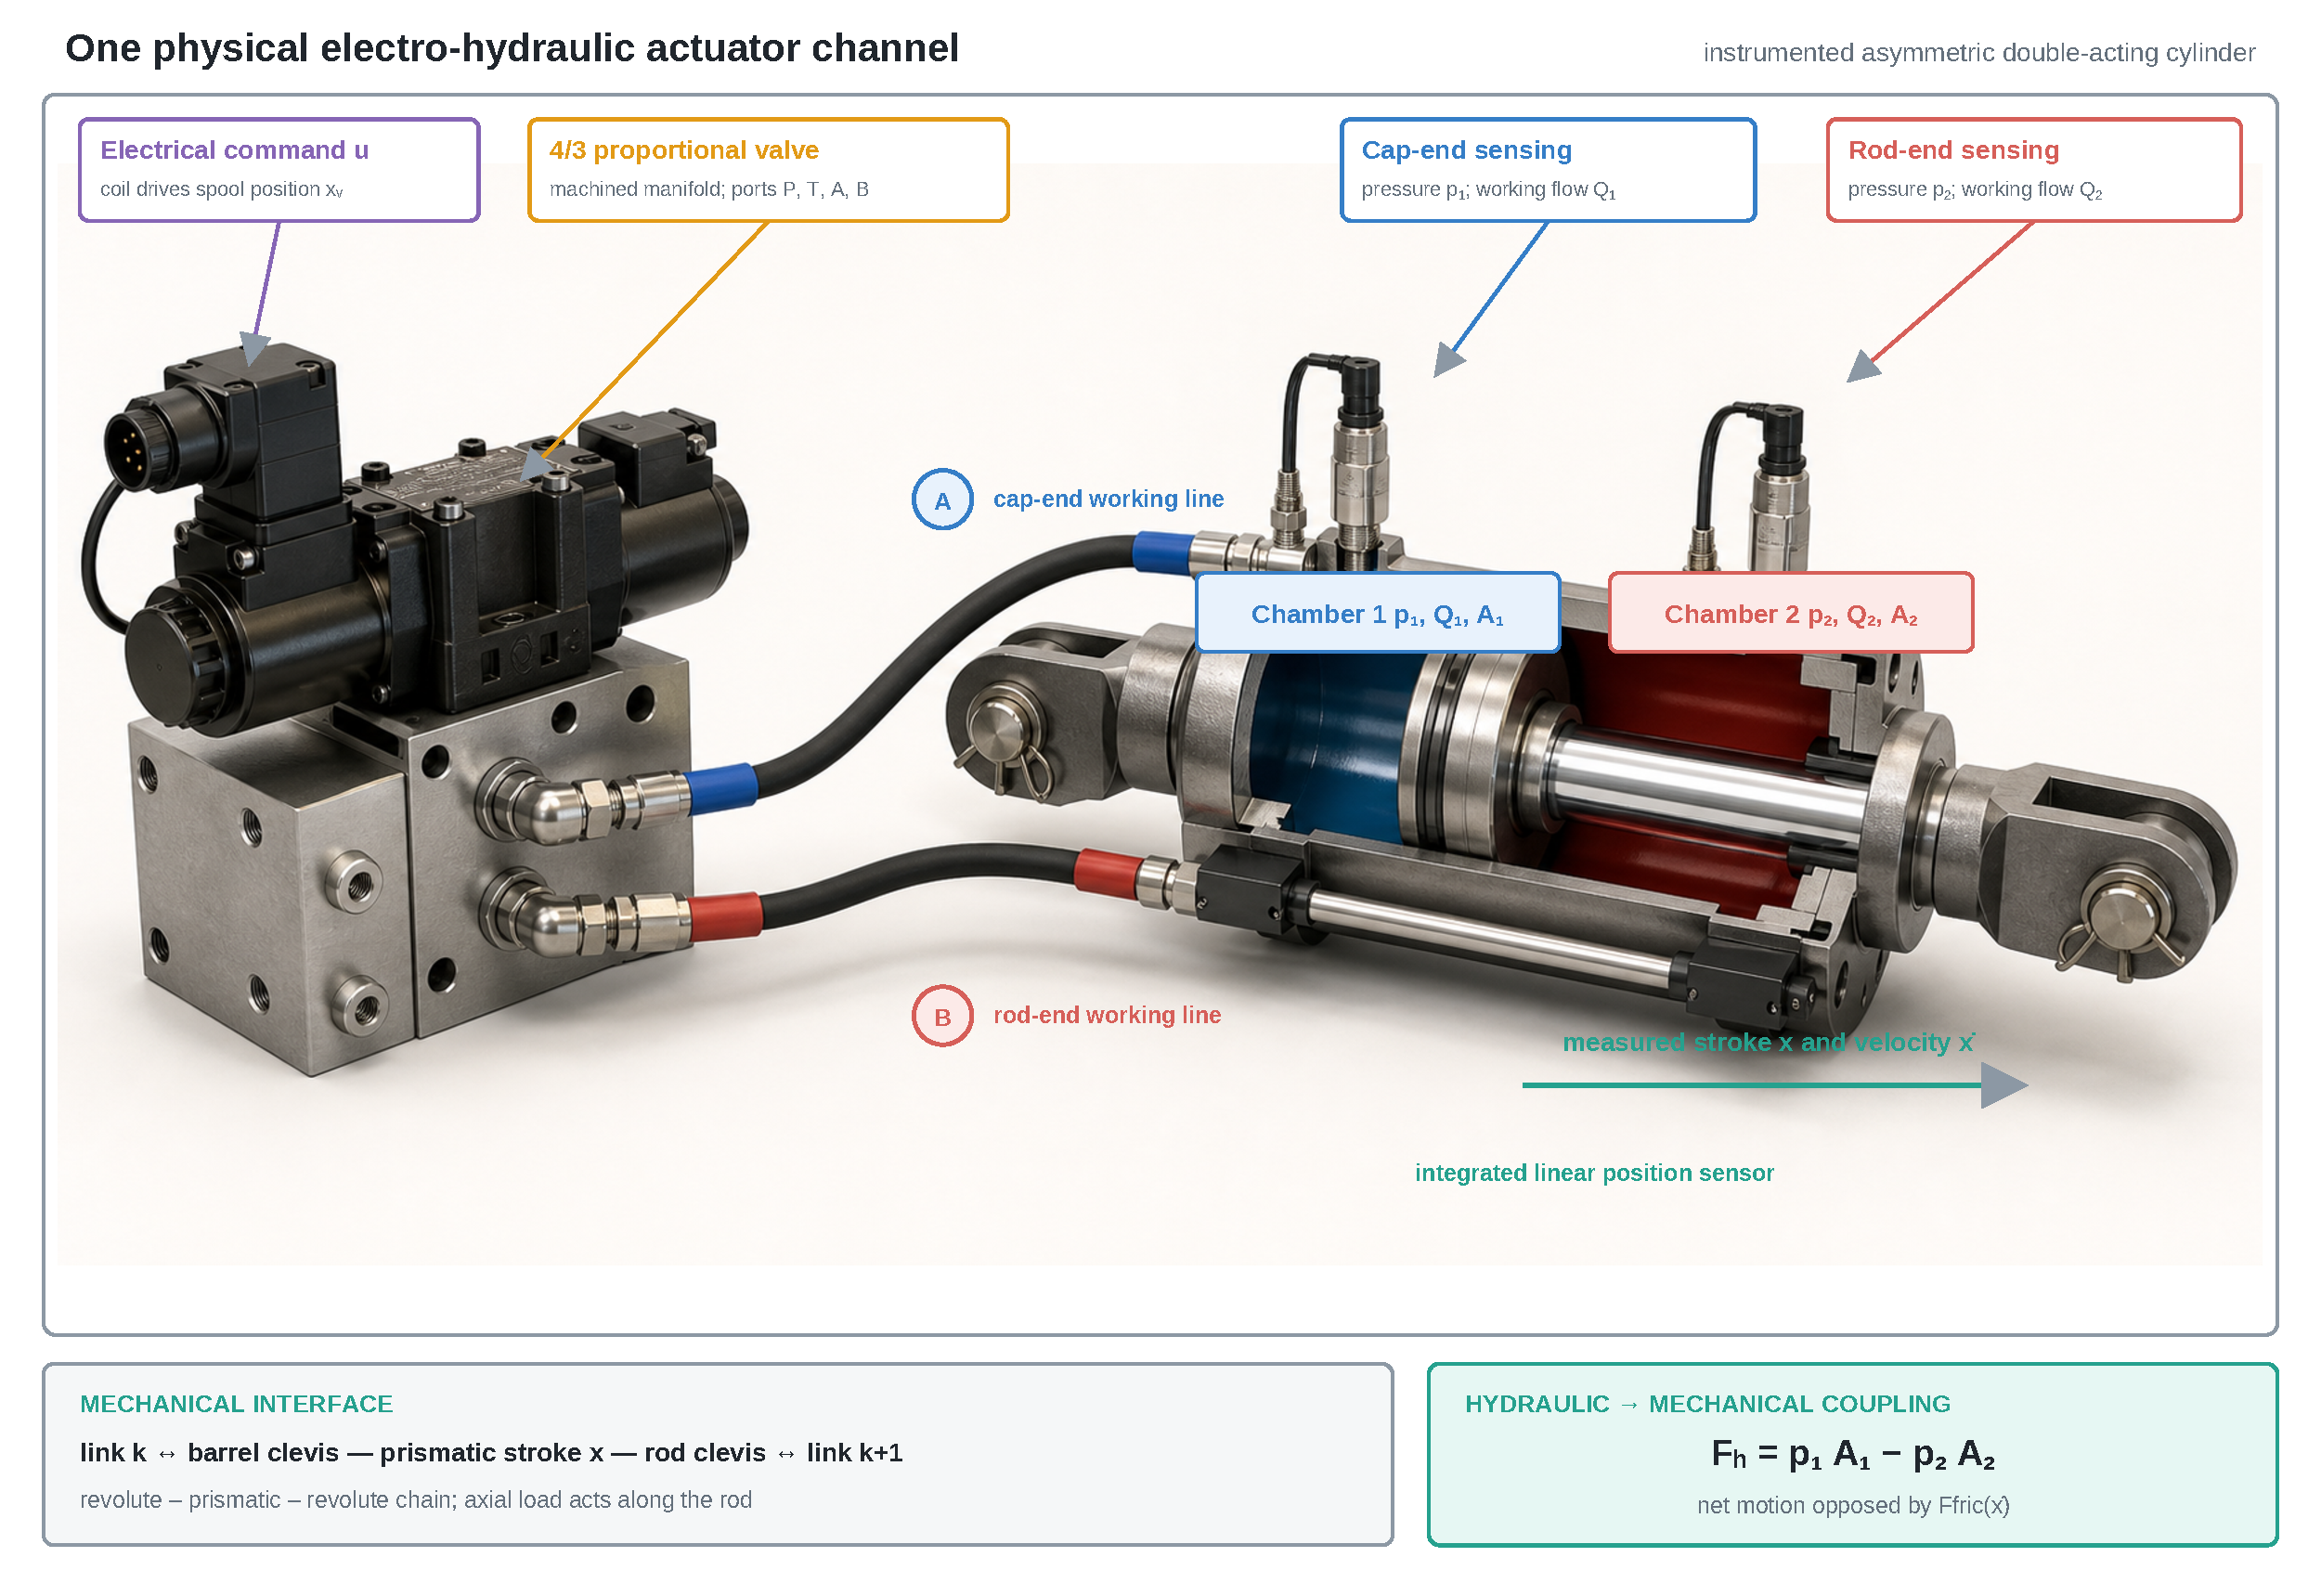
\includegraphics[width=\textwidth]{images/fme500_actuator_channel_detailed}
  \caption{One electro-hydraulic actuator channel, split into the
  upper mechanical interface and the lower hydraulic interface that
  Sections~\ref{sec:sys:kinematics} and~\ref{sec:sys:simscape}
  describe. Top: barrel and rod are rigid bodies connected to the
  adjacent links through a revolute--prismatic--revolute joint chain
  whose prismatic coordinate is the stroke $x$. The prismatic joint is
  the translational interface that exchanges the axial force $F_h$
  against the motion $x, \dot{x}$, opposed by the friction
  $F_{\mathrm{fric}}(\dot{x})$. Bottom: the asymmetric double-acting
  cylinder, with chamber pressures and flows $(p_1, Q_1)$ and
  $(p_2, Q_2)$ routed to ports A and B of the 4/3 proportional
  directional valve, which is driven by the command $u$ through the
  first-order spool lag and connected to the shared supply and return
  rails of Figure~\ref{fig:sys:schematic}. The legend, variable table,
  and force identity use the same notation as the continuity equation
  \eqref{eq:sys:continuity} and the $F_h$ identity of
  Section~\ref{sec:sys:simscape}.}
  \label{fig:sys:actuator-channel}
\end{figure}

Figure~\ref{fig:sys:schematic} shows the assembled plant at system
level. The hydraulic side is deliberately physical rather
than phenomenological. Supply comes from a fixed-displacement pump
driven at variable speed ($Q_p = D_p\,\omega$), buffered by a
gas-charged accumulator (polytropic gas model) and protected by a
pressure-relief valve, so supply pressure is a dynamic quantity that
sags under simultaneous demand and clips under load spikes. Each of the four
actuators is a 4/3 proportional directional valve driving an
asymmetric double-acting cylinder.
Figure~\ref{fig:sys:actuator-channel} details one such channel, from
the rigid-body assembly of barrel and rod through the
mechanical--hydraulic coupling interface down to the valve, the
chambers, and the measured feedback signals. The chamber pressures
follow the continuity equations
%
\begin{equation}
  \label{eq:sys:continuity}
  \dot{p}_1 = \frac{E_{\mathrm{eff}}}{V_1(x)}
    \bigl( Q_1 - A_1 \dot{x} - C_{\mathrm{leak}}(p_1 - p_2) \bigr),
  \qquad
  \dot{p}_2 = \frac{E_{\mathrm{eff}}}{V_2(x)}
    \bigl( -Q_2 + A_2 \dot{x} + C_{\mathrm{leak}}(p_1 - p_2) \bigr),
\end{equation}
%
with stroke-dependent chamber volumes $V_{1,2}(x)$ that include the
line dead volumes, piston areas $A_1 \neq A_2$, and laminar internal
leakage $C_{\mathrm{leak}}$. The effective bulk modulus accounts for
entrained air through
%
\begin{equation}
  \label{eq:sys:bulk}
  E_{\mathrm{eff}}(p) =
  \left( \frac{1}{E_f} + \frac{\alpha}{p} \right)^{-1},
\end{equation}
%
so fluid stiffness itself is pressure dependent, weakest where precise low-pressure positioning is attempted. Valve flow follows the
orifice law of Chapter~\ref{chap:fundamentals}
(Section~\ref{sec:fund:actuation-chain}), and the spool is not an instantaneous
gain but a first-order lag, $\dot{x}_v = (u - x_v)/\tau_v$, so command
transients are bandwidth limited. The net piston force
$F_h = p_1 A_1 - p_2 A_2 - F_{\mathrm{fric}}(\dot{x})$ feeds back into
the mechanism through the virtual-work mapping of
Section~\ref{sec:sys:kinematics}, closing the bidirectional coupling:
mechanical loads shape pressure transients, and pressure transients
shape motion. Because cylinder-induced stiffness is high while
rigid-body motion is slow, the coupled equations are stiff, and the
model runs under a variable-step implicit solver. This stiffness is the
computational reason the Simscape plant cannot serve as an RL training
environment (Section~\ref{sec:fund:sim-data-source}).

\subsection{Validated Scope of the Model}
\label{sec:sys:simscape-validation}

A plant model intended as a data generator must be trusted for its
\emph{dynamics}, not just its geometry. The validation strategy in the
modeling study was control-based: a fixed integral backstepping
controller at $\unit[0.01]{s}$ was applied as a standardized excitation
instrument, and the emergent behavior of the closed loop was examined
as the physical parameters varied. The headline experiment sweeps the
effective bulk modulus over $\beta \in \{0.5, 1.0, 1.5, 2.0\}\,
\mathrm{GPa}$, the physically meaningful range from strongly aerated to
very stiff fluid, with all controller gains held constant.
Figure~\ref{fig:sys:bulkmod} shows the result re-plotted from the
study's measurements. Actuation delay behaves as hydraulic intuition
demands: the valve-to-joint delay of the heavy slew axis falls from
about $\unit[0.85]{s}$ at $\unit[0.5]{GPa}$ to $\unit[0.65]{s}$ at
$\unit[2.0]{GPa}$, the system-level delay index from roughly
$\unit[0.45]{s}$ to $\unit[0.35]{s}$, and the improvement saturates
beyond $\unit[1.5]{GPa}$, where mechanical inertia rather than fluid
compliance limits the response. Task-space tracking error falls
monotonically with stiffer fluid, by about 11\,\% over the sweep. The
model, in other words, reproduces the ``stiff yet oscillatory''
character of real hydraulic machinery and responds to parameter changes
in the physically expected direction, which is the property that Chapter~\ref{chap:data} exploits when it randomizes these same
parameters to generate plant families.

\begin{figure}[tb]
  \centering
  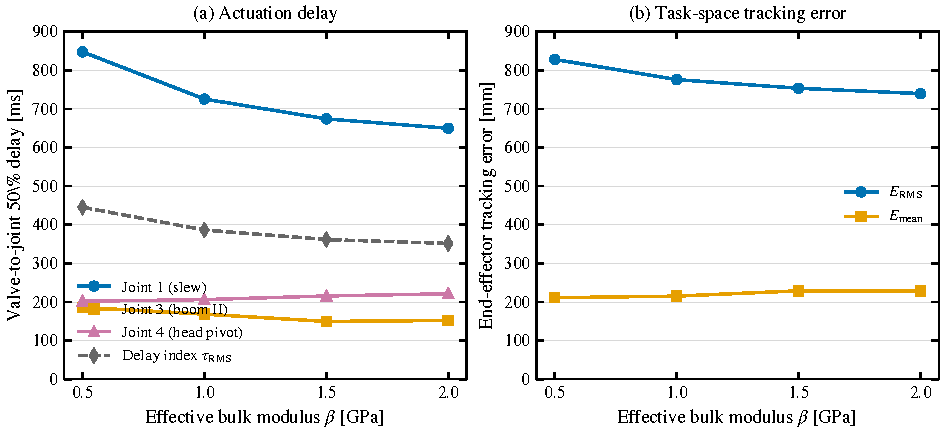
\includegraphics[width=\textwidth]{images/ch3_bulk_modulus_sensitivity}
  \caption{Sensitivity of the Simscape plant to the effective bulk
  modulus, measured in the preceding modeling study.
  (a)~Valve-to-joint 50\,\% delays of
  the dominant axes and the RMS delay index; (b)~end-effector tracking
  error of the fixed validation controller. Softer fluid slows the arm
  and degrades tracking. The effect saturates beyond
  $\unit[1.5]{GPa}$.}
  \label{fig:sys:bulkmod}
\end{figure}

Three limitations are carried forward honestly. The model is a single
machine: manufacturing spread enters only through the deliberate
parameter randomization of Chapter~\ref{chap:data}, not through
measured variation. Thermal dynamics are not modeled. Temperature
effects are represented indirectly through the parameters they act on
(bulk modulus, friction). And the logged rod-force channel failed a
piston-area consistency audit on the current export
(Section~\ref{sec:models:rom}), so force is treated as unreliable
supervision throughout the thesis.

\section{IsaacLab Environment}
\label{sec:sys:isaaclab}

Policy training, adaptation-data collection, and every closed-loop
result in this thesis run in IsaacLab~\cite{mittal2023orbit} on the
GPU-parallel PhysX engine. The same CAD-derived mechanism enters here as
a USD articulation: the Unimog carrier with wheels, the five arm links,
and the four cylinders represented as prismatic actuator joints, with
self-collisions enabled and the solver configured for the long-chain
mechanism. Figure~\ref{fig:sys:unimog} renders that articulation
directly from the asset the environment loads. The complete machine is shown once, because the arm-only views of
Section~\ref{sec:sys:platform} do not convey the geometry that makes
this task what it is: the boom is mounted on the front of a road-going
carrier and reaches out to one side, so the cutter works several metres
from the vehicle that carries it while that vehicle keeps driving. Every
lever arm, every reaction force on the chassis, and the entire reason
the vehicle's motion must be treated as part of the plant follow from
this arrangement.

\begin{figure}[tb]
  \centering
  \begin{subfigure}[b]{.56\linewidth}
    \centering
    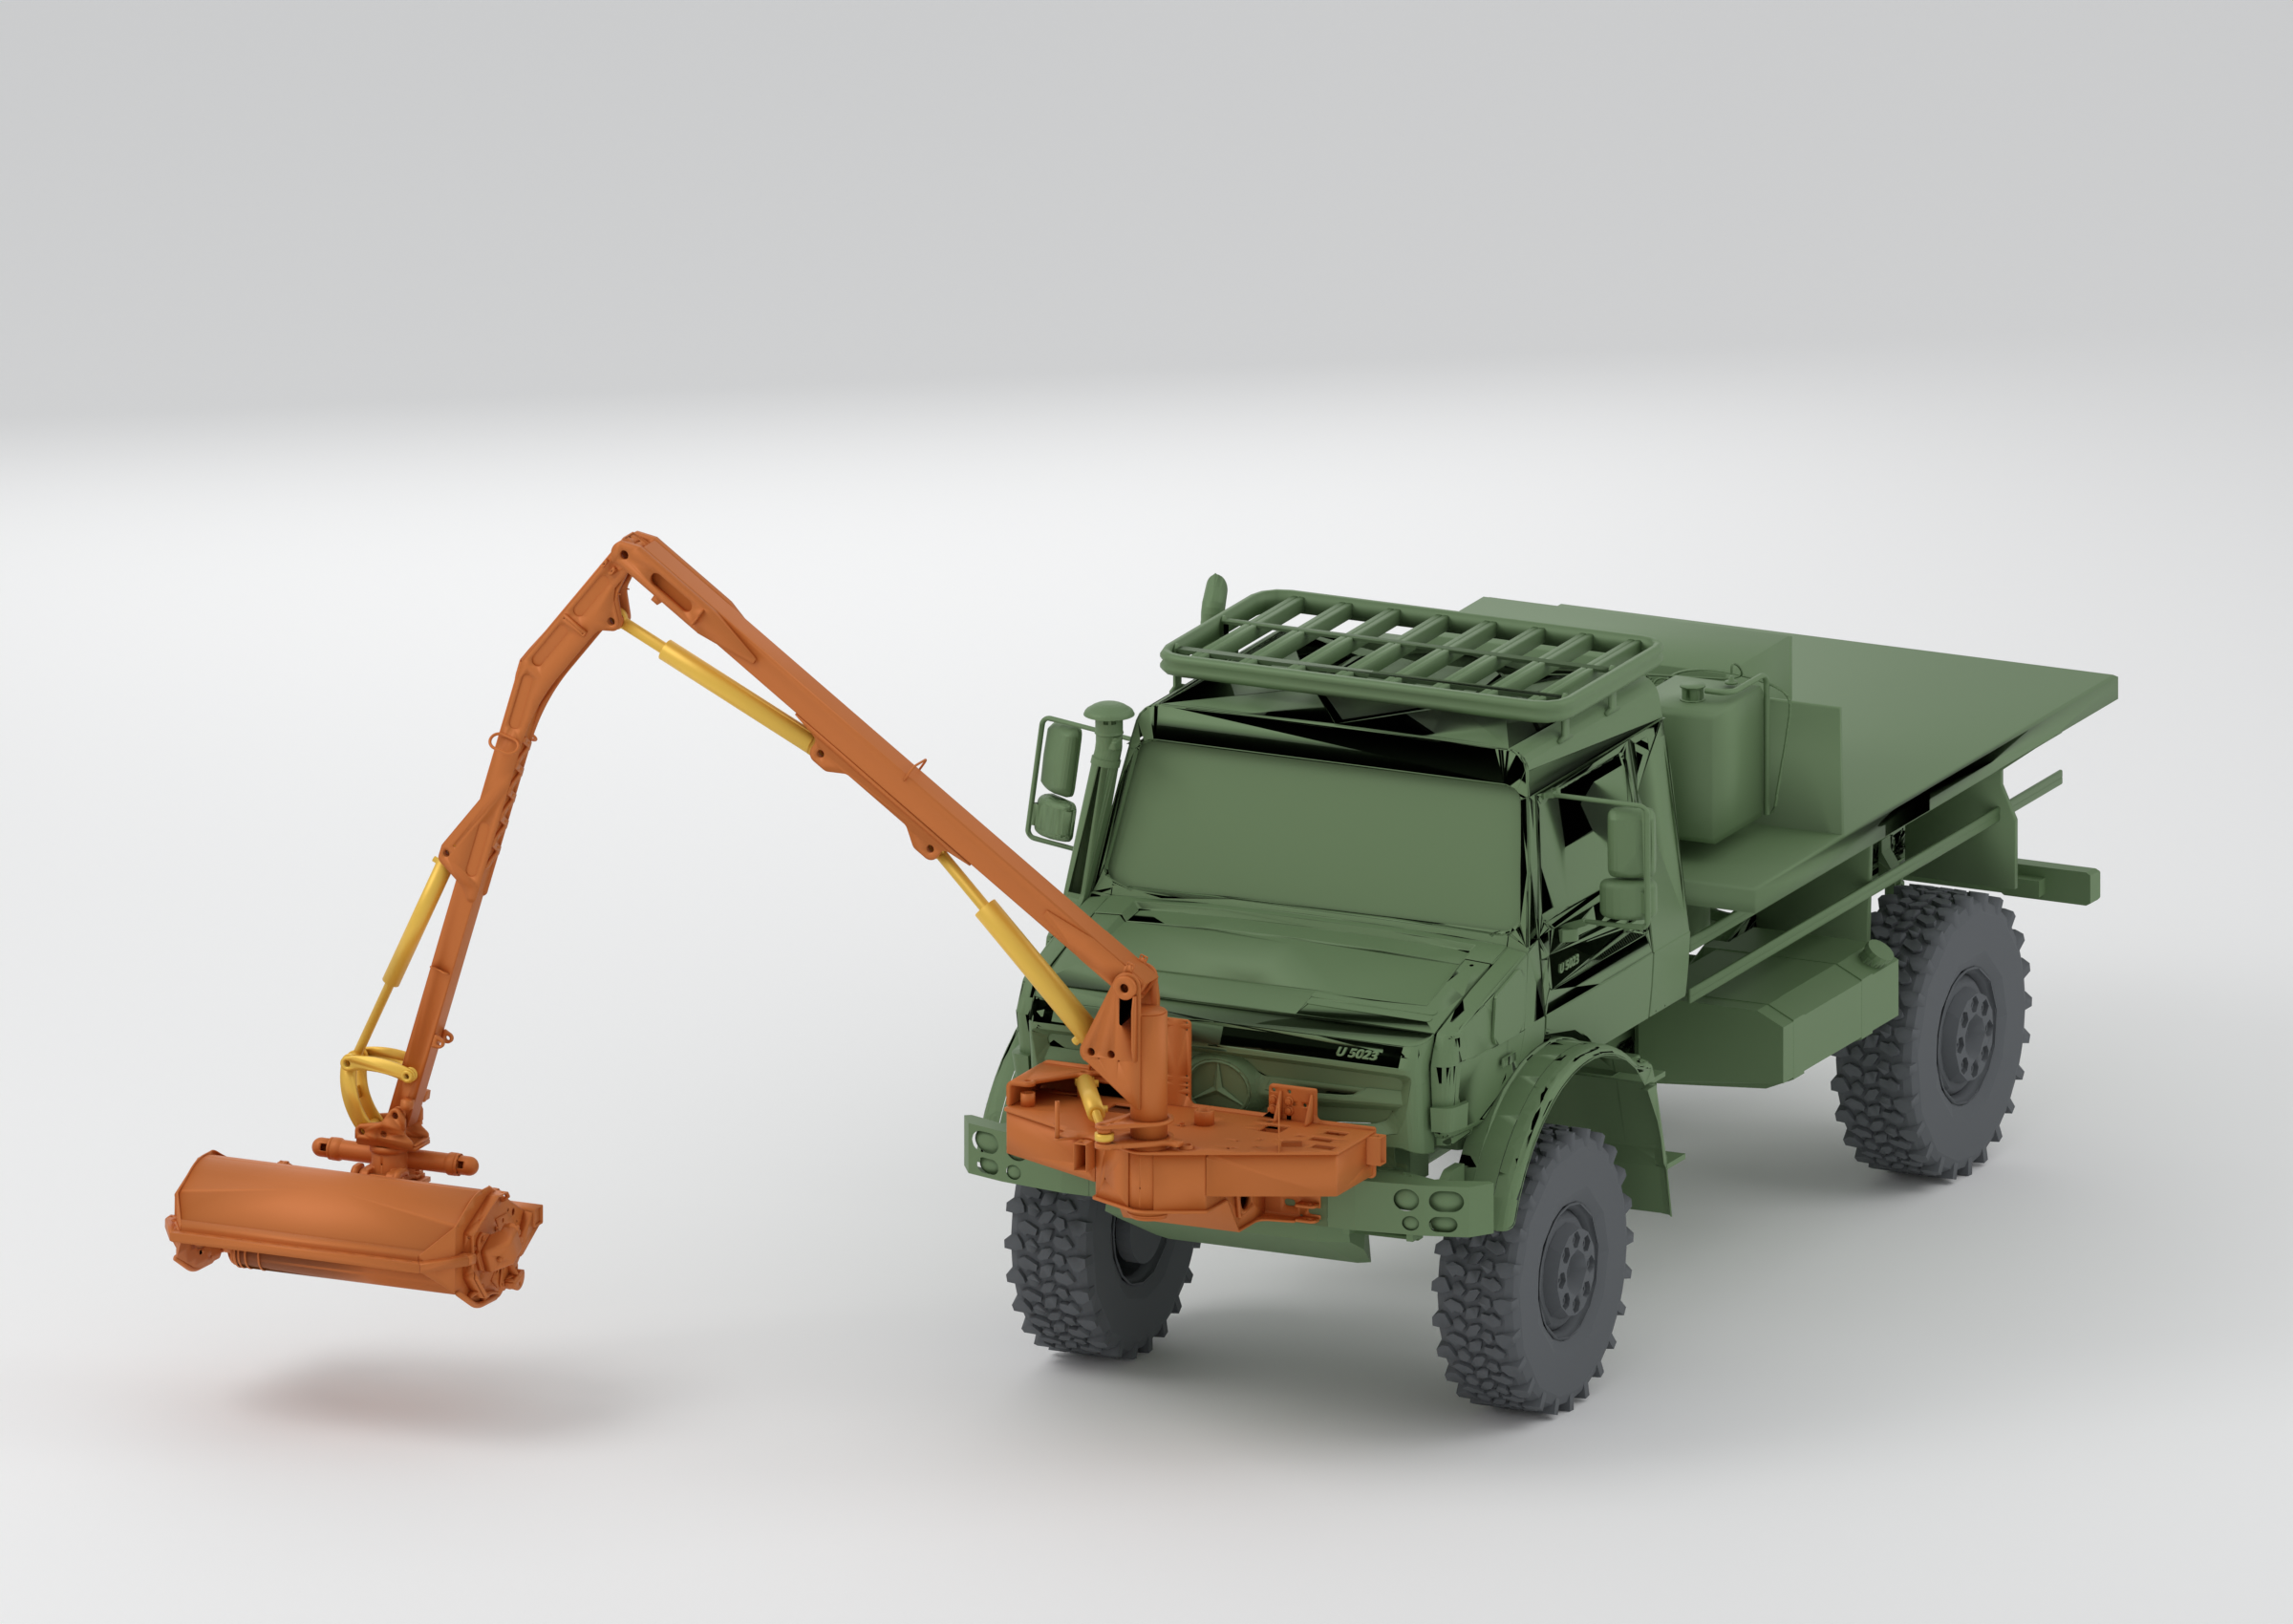
\includegraphics[width=\linewidth]{images/unimog_mulag_iso}
    \caption{}
    \label{fig:sys:unimog-front}
  \end{subfigure}
  \hfill
  \begin{subfigure}[b]{.42\linewidth}
    \centering
    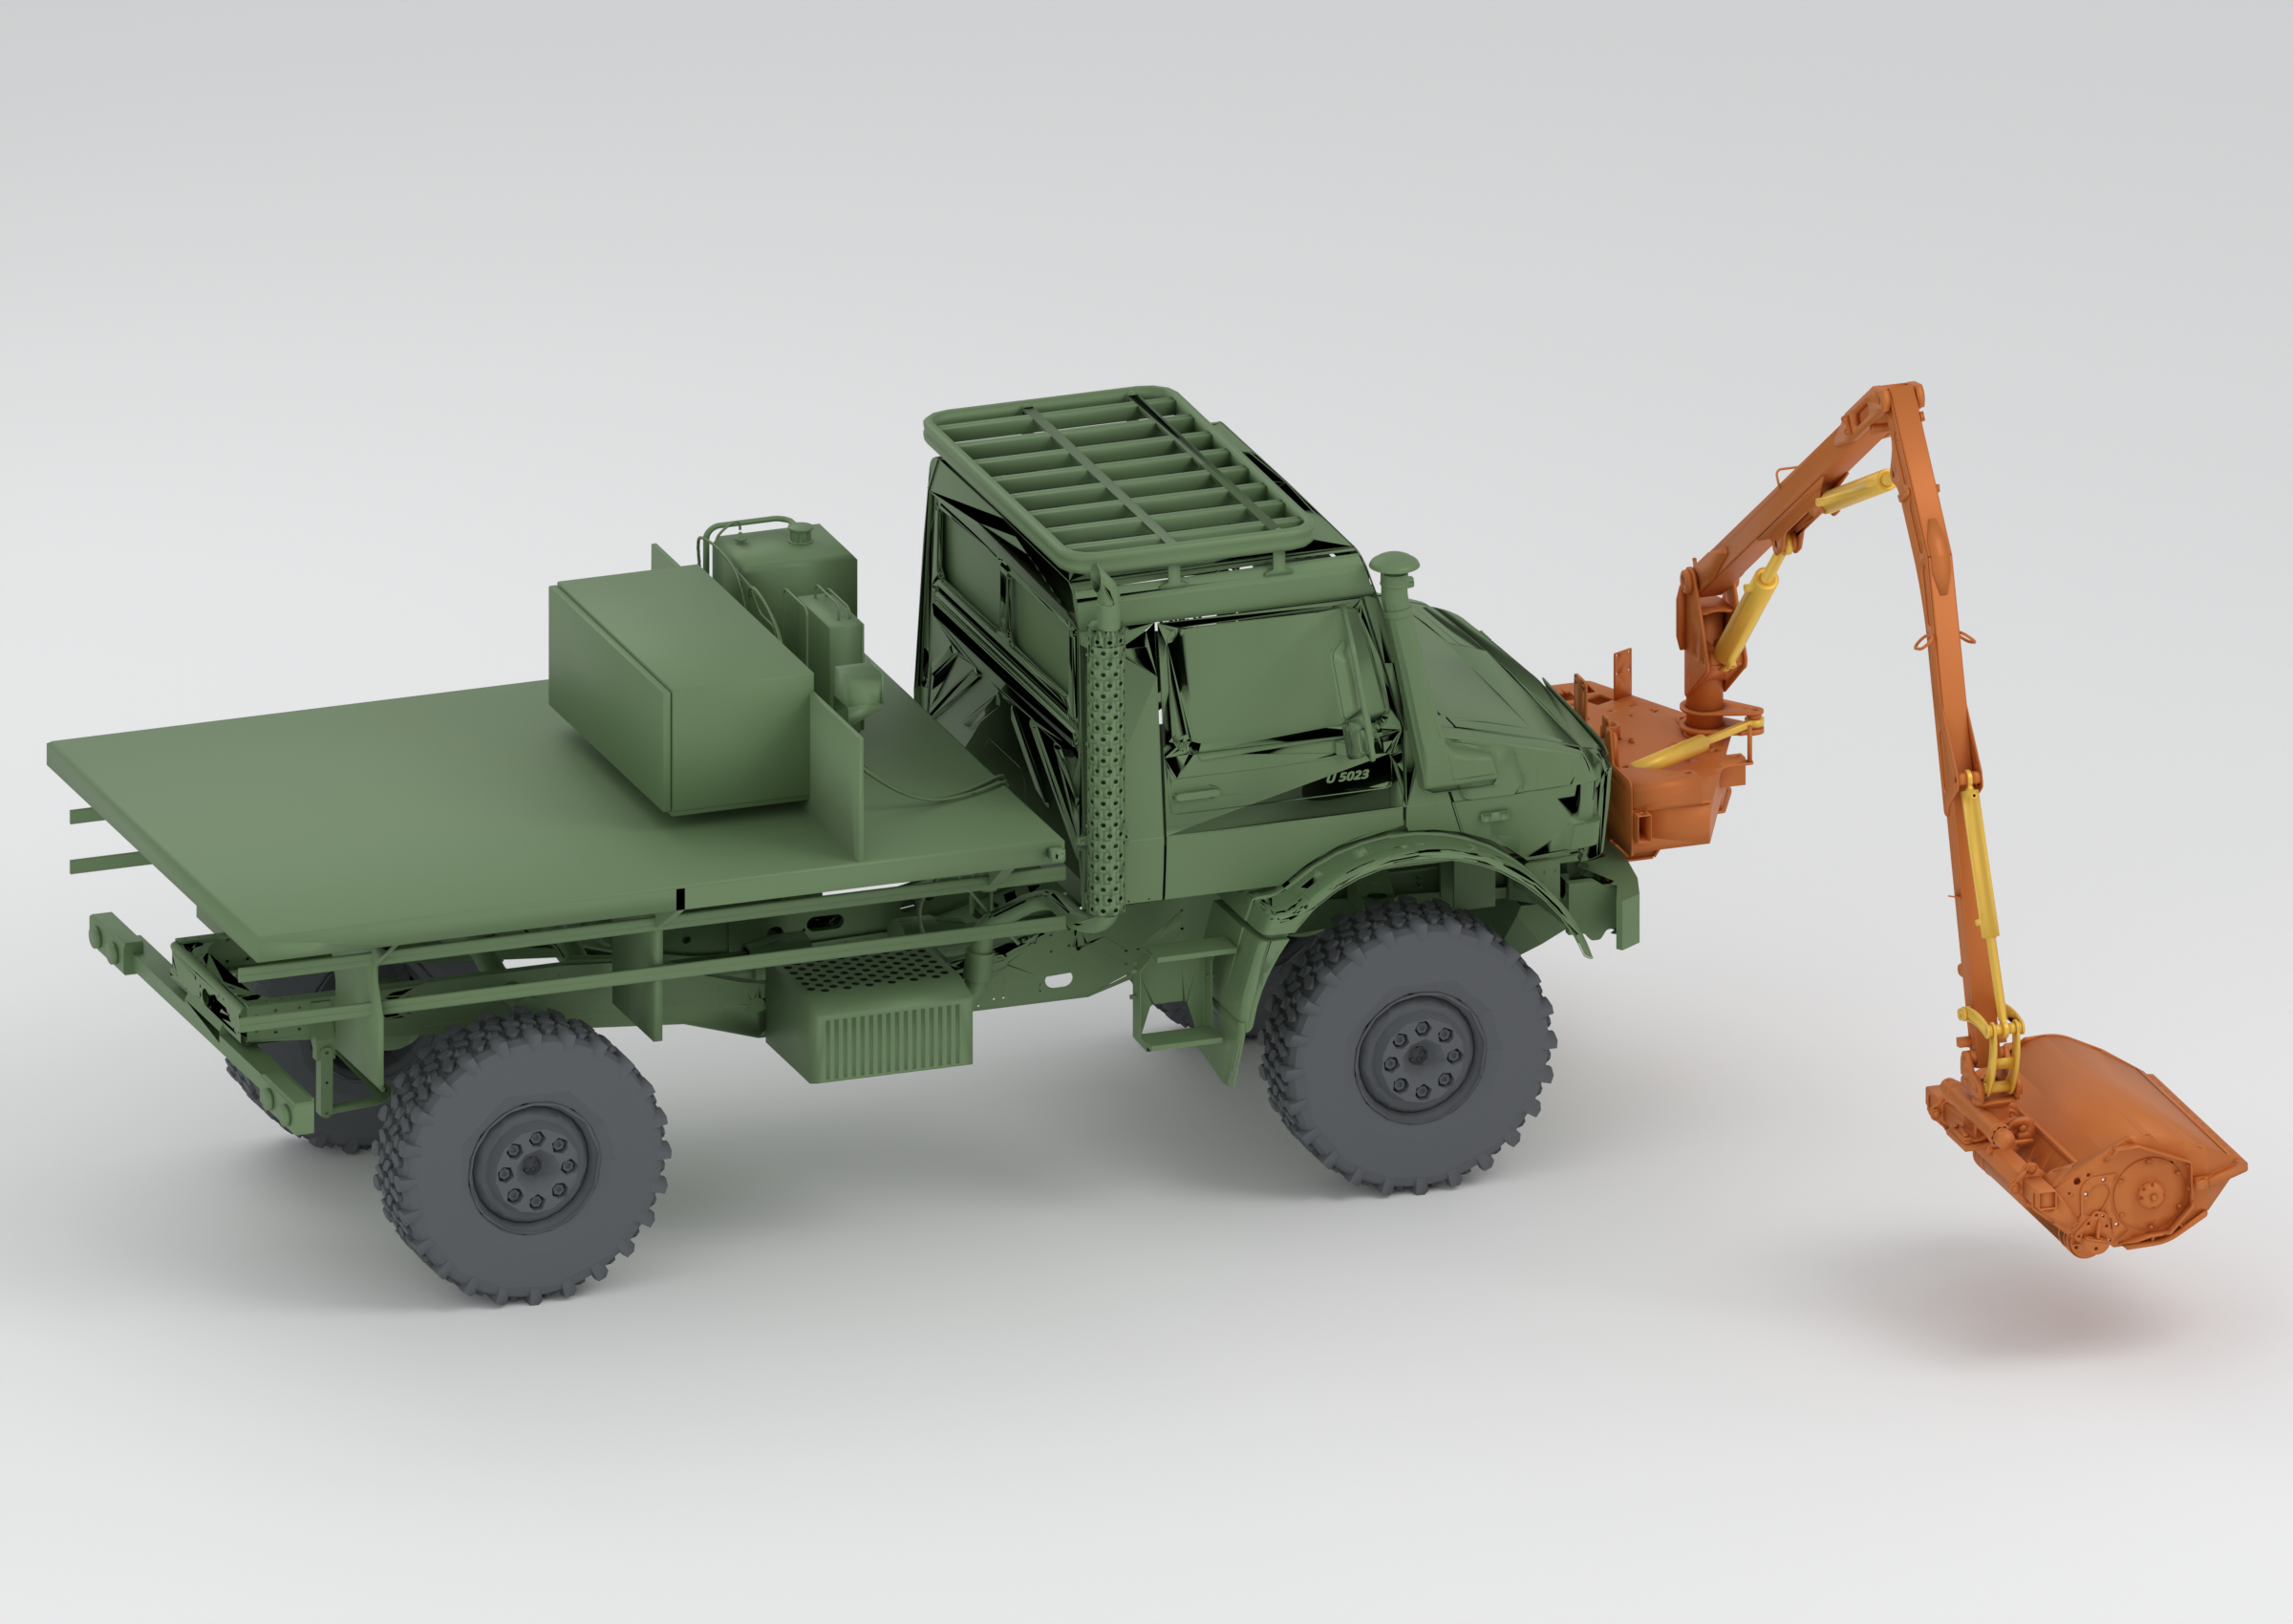
\includegraphics[width=\linewidth]{images/unimog_mulag_rear}
    \caption{}
    \label{fig:sys:unimog-rear}
  \end{subfigure}
  \caption{The complete simulated machine, rendered directly from the
  USD articulation that the IsaacLab environment loads: the Unimog implement carrier with the MULAG FME~500 boom mounted on its front
  frame and the flail head deployed to the side. (a)~Front three-quarter
  view; (b)~rear three-quarter view of the same configuration. The four
  hydraulic cylinders are highlighted in orange, following the
  convention of Figure~\ref{fig:sys:cad}. This is the mechanism, the
  carrier, and the mounting geometry exactly as PhysX simulates them.
  The hydraulics are not present here and enter only through the learned
  actuator models.}
  \label{fig:sys:unimog}
\end{figure}

The full hydraulic model does not run inside these environments, for the
computational reasons of Section~\ref{sec:fund:sim-data-source}. Its
behavior enters only through the learned actuator representations
sitting between the controller and the PhysX cylinder targets.

\subsection{Simulation and Control Rates}
\label{sec:sys:timing}

Four different clocks run in this system, and reporting any one of them
as ``the control frequency'' misstates the interface. They are listed in
Table~\ref{tab:sys:rates}. The physics step is $\unit[1/120]{s}$ with a
control decimation of two, so the policy observes and acts at
$\unit[60]{Hz}$ ($\unit[16.7]{ms}$). The learned actuator models keep
the native $\unit[0.05]{s}$ transition they were identified on: three
consecutive control steps make one model tick, so a learned-model
prediction is issued once every three policy steps and the resulting
motion is distributed over the intervening PhysX updates as held
increments. Nothing is interpolated onto the model grid, and the
learning samples of Chapter~\ref{chap:data} use exactly those
$\unit[50]{ms}$ transitions at control indices $0, 3, 6, \dots$. A
model asked to predict across a mismatched interval is a silent
$\unit[33]{\%}$ error in the quantity it is supposed to supply. The AAM
of Chapter~\ref{chap:models} updates on the same $\unit[50]{ms}$ model
grid from a causal history window, and logging runs at the control rate.

\begin{table}[tb]
  \centering
  \caption{The four rates of the simulated system. They are reported
  separately throughout the thesis; ``the control frequency'' is not a
  well-defined quantity here.}
  \label{tab:sys:rates}
  \small
  \begin{tabular}{lll}
    \toprule
    Layer & Step & Rate \\
    \midrule
    PhysX physics                & $\unit[1/120]{s}$   & $\unit[120]{Hz}$ \\
    Policy / control (decimation 2) & $\unit[1/60]{s}$ & $\unit[60]{Hz}$ \\
    Learned actuator model (3 control steps) & $\unit[0.05]{s}$ & $\unit[20]{Hz}$ \\
    AAM latent update            & $\unit[0.05]{s}$    & $\unit[20]{Hz}$ \\
    \bottomrule
  \end{tabular}
\end{table}

\subsection{Environment Configuration Details}

Three environment details cost real debugging time and are recorded
here so they need not be rediscovered. First, the articulation root of
the arm sits about $\unit[1.11]{m}$ above the wheel contact plane, so
the vehicle must spawn with its root at $z = \unit[1.26]{m}$. Spawning
at ground height buries the truck to its axles and silently changes
every contact force. Second, cylinder actuation uses PhysX position
targets, and the target must be integrated in \emph{reference} space,
accumulating commanded increments, rather than re-anchored each step to
the measured position: re-anchoring lets gravity sag wash out every
commanded increment, removing the policy's authority entirely. Third,
the vehicle's forward motion is \emph{scripted} rather than driven
through the wheels: the chassis is advanced kinematically along the road
at the commanded speed and its lateral position and heading are held by
a planar fixture. This is not a convenience. The authored tyres and
suspension of this asset do not produce usable traction in PhysX, and
leaving the chassis free turns arm reaction forces into slow drift and
sway that contaminate every task-space error. The residual sway the
fixture has to remove is itself measured and gated
(Section~\ref{sec:sys:evaluation-criteria}) rather than assumed to be
zero.

\section{The Verge-Following Task}
\label{sec:sys:task}

\subsection{Task Definition}

The primary task of this thesis, and the one every reported control
result is measured on, is verge following with the vehicle in motion.
The truck drives along the road at a constant speed of $\unit[4]{km/h}$
in the development configuration, reduced to $\unit[2]{km/h}$ for the
final \ppoROM{} task of Section~\ref{sec:ctrl:ppo-rom}, where the strip
is lengthened to $\unit[26]{m}$. Meanwhile the
four-cylinder arm reaches over the embankment and holds the cutter on
the verge centre line: near the target cut height, in ground contact,
head down, and inside the mechanical travel limits. Tracking the line is
the objective. The terrain is a \emph{disturbance} that makes tracking
nontrivial, not an obstacle course to be negotiated, and its height
profile is randomized per environment so that no policy can memorize one
ground surface.

Reference paths are drawn from eleven families ( \texttt{straight},
\texttt{lateral\_sine}, \texttt{s\_curve}, \texttt{random\_spline},
\texttt{offset\_return}, \texttt{boom\_sweep}, \texttt{lateral\_chirp},
\texttt{double\_s\_curve}, \texttt{lane\_change\_hold},
\texttt{gaussian\_slalom}, and \texttt{fourier\_meander}),
which span
a range of lateral demand rather than a single nominal line. Because
aggregate scores can hide one impossible family behind ten easy ones,
the acceptance criteria of
Section~\ref{sec:sys:evaluation-criteria} are evaluated at the
\emph{worst} family and the \emph{worst} terrain mesh rather than pooled.

\subsection{Task Feasibility and Plant Capability}
\label{sec:sys:capability}

One finding governs the design of everything above, and it is stated
here because it is a property of the plant rather than of any
controller. The action contract commits at most $\unit[4]{mm}$ of
cylinder travel per step on cylinders~1--3
(Chapter~\ref{chap:control}), and over the interval across which that
increment is committed this bounds the lateral cutter rate at
%
\begin{equation}
  \label{eq:sys:rate-ceiling}
  v_{\mathrm{lat}}^{\max} \approx \unit[0.200]{m/s}.
\end{equation}
%
\todo{confirm the exact interval used in the maintained figure: the
$\unit[0.200]{m/s}$ ceiling is quoted as $\unit[4]{mm}/\unit[20]{ms}$,
while the environment's control step is $\unit[1/60]{s} =
\unit[16.7]{ms}$ (Table~\ref{tab:sys:rates}), which would give
$\unit[0.24]{m/s}$. Fix one and propagate.}
At the settings used before this was measured, nine of the
eleven path families demanded more lateral rate than that, one of them
(\texttt{boom\_sweep}) by a factor of $3.7$. Tracking error then
accumulates \emph{by construction}: no reward shaping, critic change, or
policy-optimization fix can recover a target the actuator cannot reach,
and indeed the privileged DLS teacher failed on those families too,
which is the diagnostic that identified the problem. The terrain and
path parameters are therefore now \emph{derived} from
\eqref{eq:sys:rate-ceiling} rather than chosen independently of it, and
a preflight check asserts the resulting feasibility before any training
run is allowed to start.

The methodological rule generalizes beyond this machine and is applied
throughout the thesis: before attributing a tracking failure to the
learning algorithm, measure whether the commanded reference is inside
the actuator's authority. A task outside the plant's capability produces the symptoms of a badly tuned policy.

\subsection{Parked Diagnostic Workflow}
\label{sec:sys:parked}

A second, older workflow is retained and must not be confused with the
task above. With the vehicle held stationary, the cutter tracks
scripted line, arc, sine, circle, and square references in free space.
This is a \emph{diagnostic} instrument for qualifying the plant and the actuator models
(step response, per-axis authority, out-and-back return error, and
Jacobian conditioning), and it is how several of the
cylinder-level checks in this thesis are performed. It is not a fourth
control stack, it is not part of the final comparison, and its numbers
are never pooled with the moving-verge statistics. Where a parked result
is reported, it is labelled as a separate diagnostic experiment.

\section{Control Architecture}
\label{sec:sys:architecture}

\begin{figure}[tb]
  \centering
  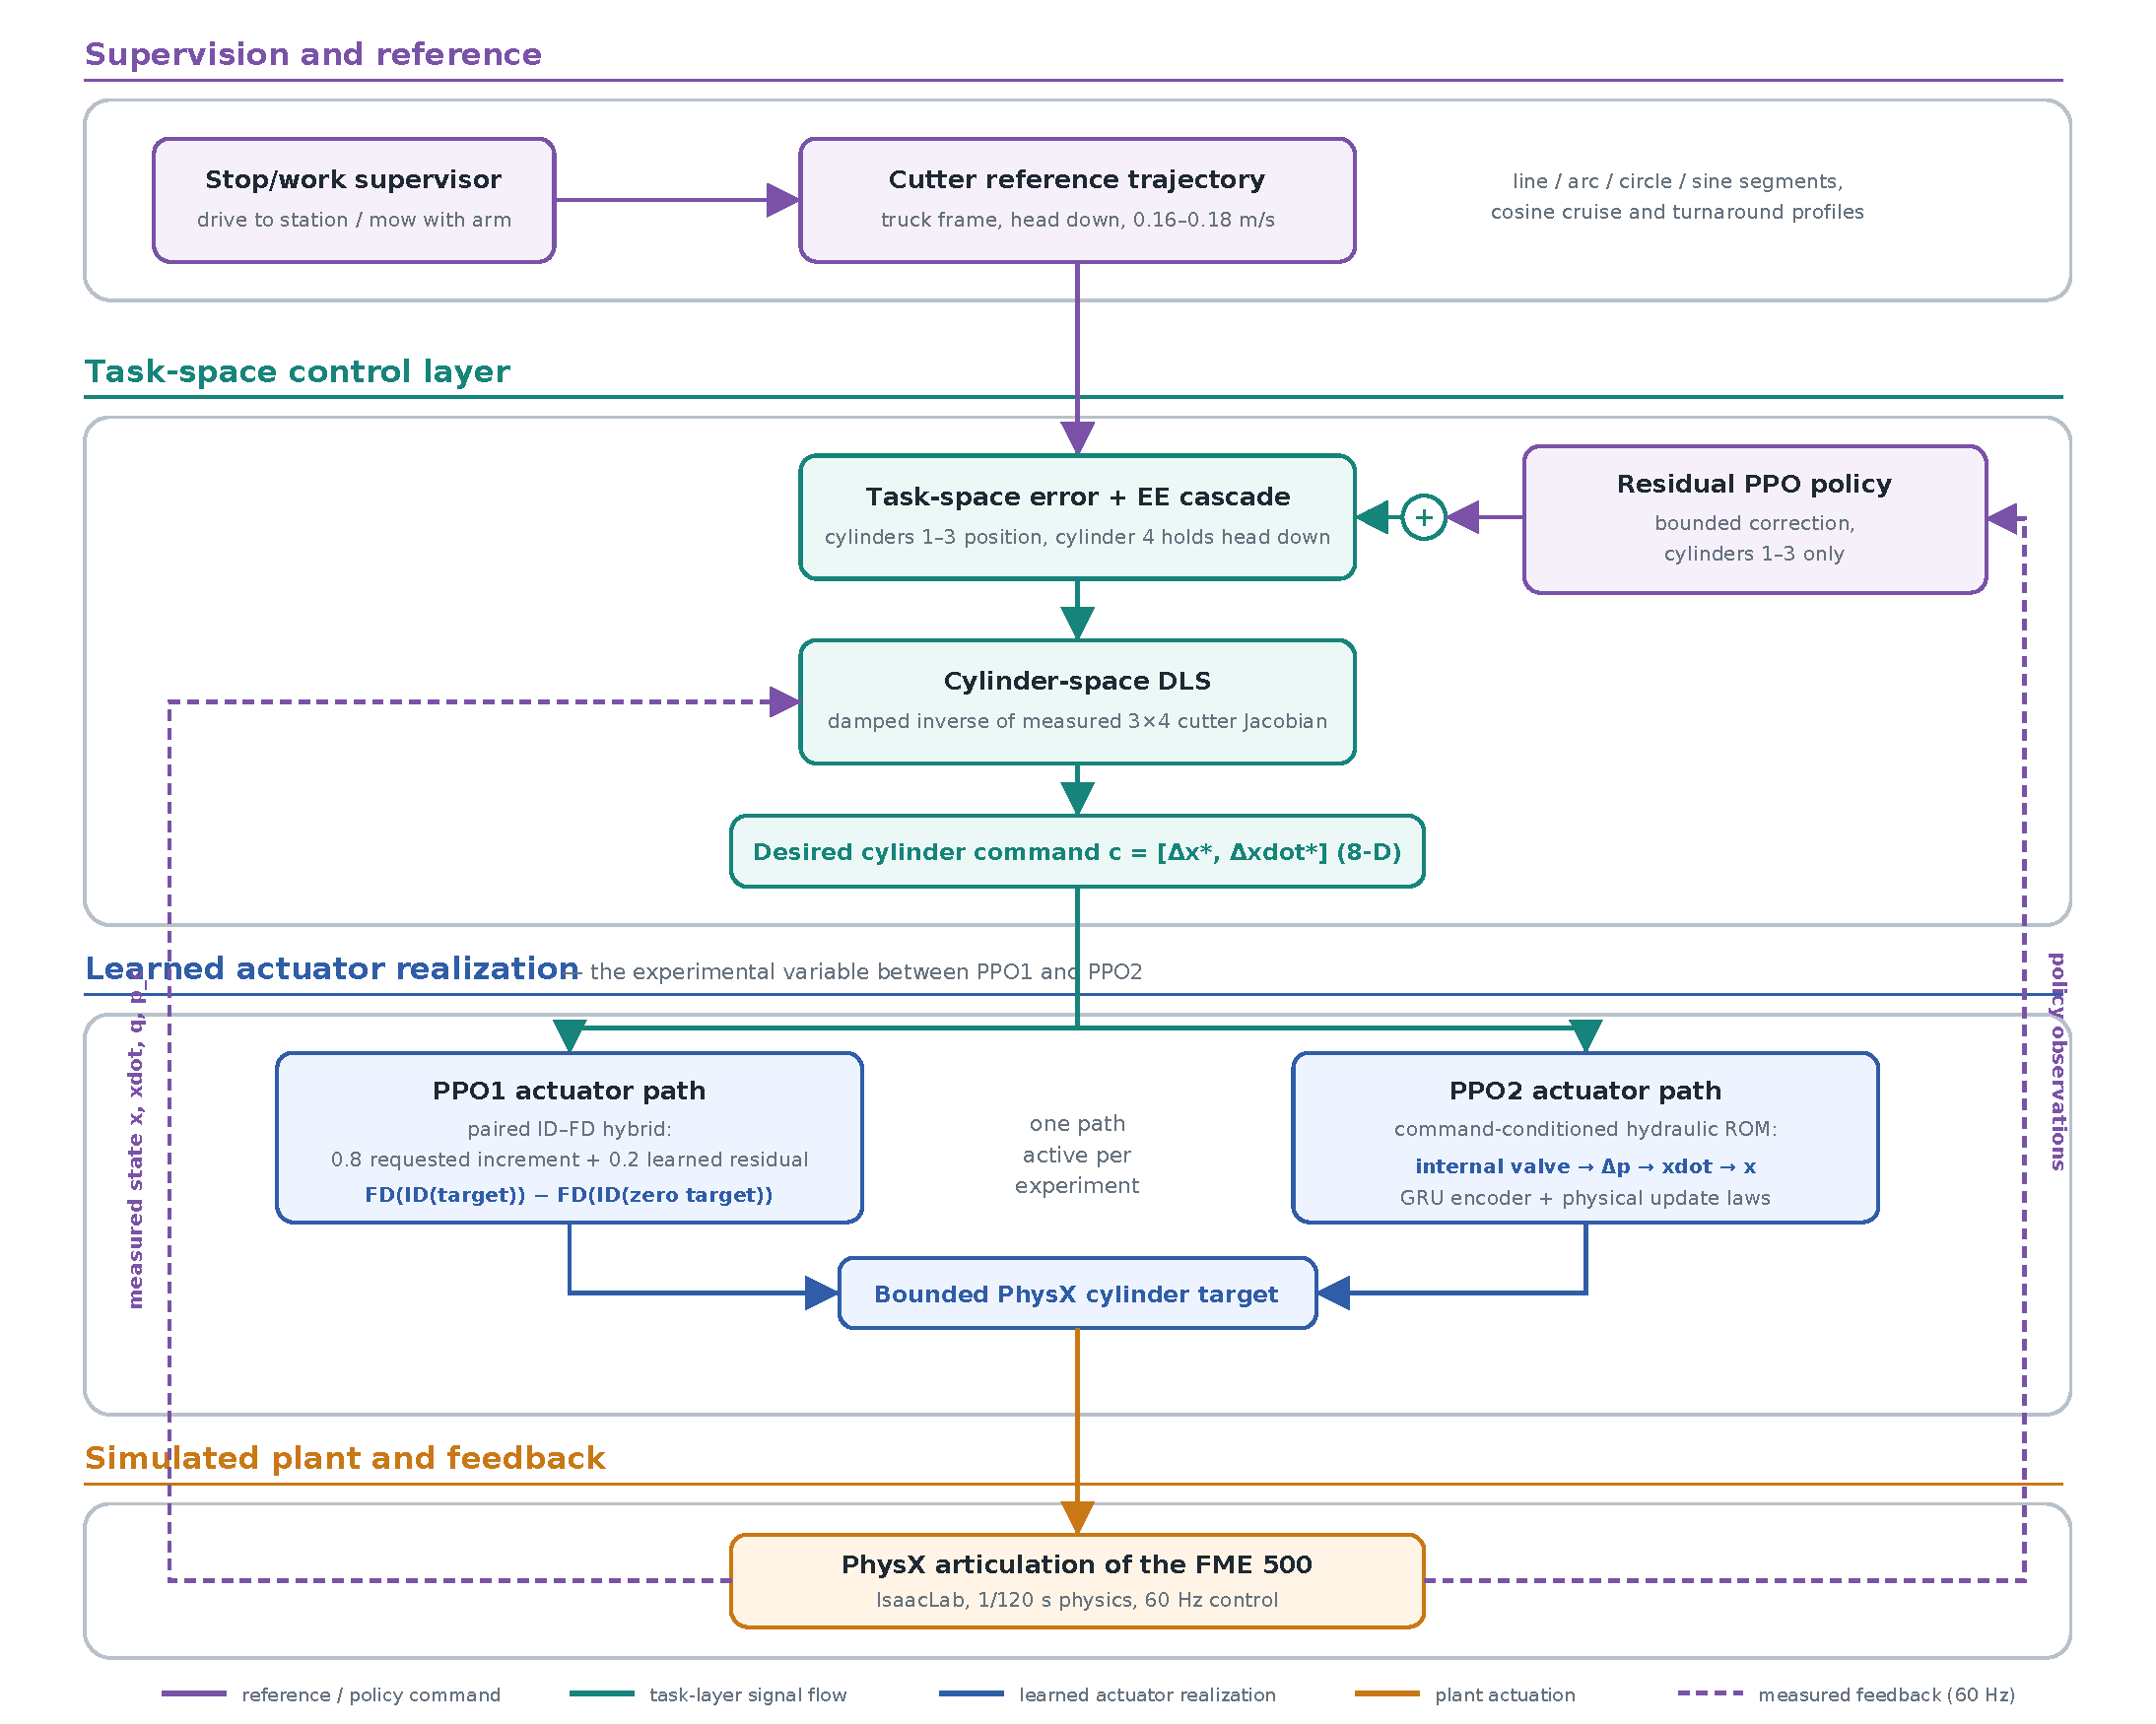
\includegraphics[width=.95\textwidth]{images/fme500_control_architecture}
  \caption{Control architecture used in all experiments, organized by
  layer. The vehicle advances along the road at constant speed and the
  reference generator supplies the verge centre line and target cut
  height in the truck frame. The policy is the task layer: a memoryless
  Gaussian MLP that observes the terrain scan, the task errors, the
  cylinder state, and the actuator's own model error, and emits the
  desired cylinder command for all four cylinders directly. The learned
  actuator layer below it is the experimental variable and the only
  thing that differs between the three stacks: the command ROM
  (\ppoROM), the frozen ID followed by the frozen strict FD
  (\ppoIDFD), or the same pair with an AAM-conditioned bounded adapter
  inserted after the ID (\ppoIDAAMFD). All three end in the same
  bounded PhysX cylinder position target. The DLS controller is drawn
  outside the deployed loop because that is where it lives: it is the
  privileged teacher used for distillation and identification, not a
  runtime layer.
  \todo{regenerate this figure: the current artwork still shows the
  stop/work supervisor and the residual-PPO summing junction.}}
  \label{fig:sys:architecture}
\end{figure}

Figure~\ref{fig:sys:architecture} assembles the pieces. The vehicle
layer advances the chassis along the road at the scripted task speed of
Section~\ref{sec:sys:task} and is not under policy control. The reference generator supplies the verge centre
line, drawn from one of the eleven path families of
Section~\ref{sec:sys:task}, together with the target cut height.

The policy is the entire task layer. It is a memoryless Gaussian MLP
that reads the forward terrain profile, the cut-height and lateral
errors, the cylinder extensions, velocities and travel headroom, its own
previous action, the actuator's current valve command and predicted
increment, the head-down alignment and its rate, the truck speed, the
cutter contact force, a short path preview, and the actuator's standing
model error. From these it emits four normalized actions, one desired
motion command per hydraulic cylinder. It is \emph{not} a residual: no
nominal command is added to its output at runtime, and there is no
baseline controller underneath it in the deployed loop. What keeps the
commands inside the learned actuator's validated envelope is the action contract itself:
the per-step command scale, the target-lead caps, the action-rate filter,
and limit shielding, which Chapter~\ref{chap:control} specifies in full.

The damped least-squares inverse of the measured Jacobian $\bm{J}_c$
still appears twice in this thesis, but never inside the deployed loop.
It is the privileged teacher whose demonstrations the policies are
distilled from, and it is the closed-loop controller that drove the
identification runs of Chapter~\ref{chap:data}. Reporting it as a
runtime nominal layer would misdescribe the architecture and would make
every stack's result a property of a pair rather than of the policy.

Below the task layer sits the experimental variable of the whole thesis:
the actuator path that realizes the desired cylinder command. In
\ppoROM{} the command-conditioned reduced-order model realizes it and
predicts the valve internally. In \ppoIDFD{} the frozen inverse model
maps command and state to a valve command, and the frozen strict forward
model maps that valve command to the cylinder increment. In
\ppoIDAAMFD{} the same pair is used, with a small bounded adapter
inserted between them and conditioned on the AAM's inferred latent
$\latenthat$. The forward model, the policy, and the plant are
unchanged, and during warm-up or invalid AAM output the correction is
zero and the stack falls back exactly to \ppoIDFD. All three end in the
same bounded PhysX cylinder position target, and the measured state
closes the loop at the rates of Table~\ref{tab:sys:rates}.

\section{Problem Formulation}
\label{sec:sys:problem}

With the system fixed, the control problem can be stated compactly.
The vehicle advances along the road at constant speed, so the reference
is not a free trajectory in three dimensions but a verge centre line
$y_{\mathrm{ref}}(t)$ and a target cut height $h_{\mathrm{ref}}$, both
expressed in the truck frame and drawn from the eleven path families of
Section~\ref{sec:sys:task}. Writing $\bm{p}_c(t)$ for the measured
cutter-tip position and $g(\cdot)$ for the terrain height beneath it,
the two scored errors are
%
\begin{equation}
  \label{eq:sys:error}
  e_{\mathrm{lat}}(t) = p_{c,y}(t) - y_{\mathrm{ref}}(t),
  \qquad
  e_{\mathrm{cut}}(t)
    = \bigl(p_{c,z}(t) - g(\bm{p}_c(t))\bigr) - h_{\mathrm{ref}} .
\end{equation}
%
The \emph{tracking objective} is to keep $|e_{\mathrm{lat}}|$ and
$|e_{\mathrm{cut}}|$ small in mean and in the tail over complete
episodes, on every path family and on unseen terrain, while the cutter
stays in ground contact, the head stays down, and the motion remains
smooth enough not to damage the machine. The \emph{model objective},
developed in Chapter~\ref{chap:models}, is that each learned actuator
representation predict the cylinder response to its commands accurately
over one step and over recursive rollouts, with demonstrated input
authority. The \emph{robustness objective} asks that this performance
persist across the randomized plant family $\{\mathcal{P}(\factorvec)\}$
of Chapter~\ref{chap:data}. The \emph{adaptation objective} asks that
the stack conditioned on the inferred latent $\latenthat$ recover
performance on held-out factor configurations, further than the
non-adaptive stack and approaching the privileged true-latent oracle,
without degrading the nominal domain and without violating any
acceptance gate.

All objectives are subject to the same constraint set: cylinder
extensions within the ranges of Table~\ref{tab:sys:cylinders} with a
positive travel margin retained, per-step commanded increments and
target leads bounded by the action contract of
Chapter~\ref{chap:control}, valve or adapter outputs within the per-axis
limits stored in the learned checkpoints, and the head held down
throughout.

What makes this problem hard is not any single ingredient but their
conjunction, and the chapters so far have each contributed one piece of
the difficulty: the actuator chain is nonlinear and drifting
(Chapter~\ref{chap:fundamentals}), only three task directions are
controllable and the mapping into them varies with configuration
(Section~\ref{sec:sys:kinematics}), the true actuator state is not
observable at runtime (Section~\ref{sec:sys:actuation}), the reference
sits close to the plant's own rate ceiling
(Section~\ref{sec:sys:capability}), the ground is a randomized
disturbance rather than a known surface, and the high-fidelity plant
that knows the hydraulic answers is too slow to train against
(Section~\ref{sec:sys:simscape}).

\section{Evaluation Criteria at System Level}
\label{sec:sys:evaluation-criteria}

The thesis judges controllers and models by fixed, pre-registered
gates rather than by single aggregate scores, and it separates the two levels: a controller metric can hide model weakness behind
policy compensation (Section~\ref{sec:fund:rl-residual}), so model
metrics are always reported alongside.

\subsection{The Eight-Gate Task Contract}

At the \emph{system level}, acceptance is an eight-gate contract, listed
in Table~\ref{tab:sys:gates}. Each gate corresponds to something an
operator would notice: it cuts at the right height, it follows the line,
it stays on the ground, it keeps the head down, it does not slam into
the terrain, it does not shake itself apart, it does not drive into its
own travel limits, and its episodes complete.

\begin{table}[tb]
  \centering
  \caption{The eight acceptance gates. Every gate is evaluated on at
  least three distinct terrain meshes and reported at its \emph{worst}
  mesh, and the two tracking-critical gates additionally at the worst
  path family. Final claims use six held-out meshes.}
  \label{tab:sys:gates}
  \small
  \begin{tabular}{llll}
    \toprule
    Gate & Metric & Threshold & Aggregation \\
    \midrule
    Cut height        & mean $|e_{\mathrm{cut}}|$
                      & $\leq \unit[0.040]{m}$ & worst mesh \\
    Lateral tracking  & mean $|e_{\mathrm{lat}}|$
                      & $\leq \unit[0.300]{m}$ & worst mesh, worst family \\
    Ground contact    & contact fraction
                      & $\geq 0.700$ & worst mesh, worst family \\
    Head alignment    & p01 head-down alignment
                      & $\geq 0.900$ & worst mesh \\
    Hard impacts      & hard-impact step fraction
                      & $\leq 0.100$ & worst mesh \\
    Tool acceleration & p95 cutter acceleration
                      & $\leq \unit[120]{m/s^2}$ & worst mesh \\
    Cylinder headroom & minimum travel margin
                      & $\geq \unit[0.005]{m}$ & worst mesh \\
    Safety terminations & termination rate
                      & $\leq 0.080$ & worst mesh \\
    \bottomrule
  \end{tabular}
\end{table}

Three rules about \emph{how} these gates are used matter more than the
thresholds themselves, and each of them was adopted after a measured
failure of the previous practice.

\paragraph{Multi-Mesh Evaluation}
An earlier contract scored every result on a single pinned terrain seed.
When the mesh was finally varied, both the headline pass and the headline failure moved a long way:
minimum head alignment ranged
$0.9027$ to $0.9698$ across three meshes, and a checkpoint that
``passed'' by $0.0007$ on the pinned mesh failed on the others. A gate
that flips with the mesh is measuring the mesh. Results here are
therefore refused unless they are measured on at least three meshes, and
reported at the worst.

\paragraph{Gating at the Optimized Resolution}
The same earlier contract read worst-of-eleven-family minima while the
optimizer maximized a pooled mean. Across ten training blocks the mean
ground contact rose from $0.817$ to $0.870$ while the worst-family
contact never left the $0.66$--$0.75$ band: nothing was optimizing what
acceptance measured.

\paragraph{Measurement-Anchored Thresholds}
A gate that nothing can pass carries no information, and several were found in that state. The tool-acceleration limit stood at
$\unit[80]{m/s^2}$ while the environment alone, with the arm commanded
to zero, measures a p95 of $\unit[100.06]{m/s^2}$. It was re-derived to
$\unit[120]{m/s^2}$, $1.2\times$ the measured floor. The ground-contact
and hard-impact thresholds were likewise anchored just outside what the
privileged DLS teacher itself achieves, so that they separate a working
controller from a non-working one rather than separating the teacher
from perfection. Every threshold in
Table~\ref{tab:sys:gates} is therefore accompanied in the source by the
measurement that fixes it, and every reported result carries its signed
margin rather than a bare pass or fail, so that a pass by $0.0007$
cannot masquerade as a comfortable one.

\subsection{Cylinder- and Model-Level Criteria}

At the \emph{cylinder level}, the parked diagnostic workflow of
Section~\ref{sec:sys:parked} supplies step gates: clean response to
fresh $\pm\unit[10]{mm}$ commands on every axis, small terminal error on
large ($\unit[80]{mm}$) coordinated motions, and low out-and-back return
error, all without command saturation. Model-level criteria
(one-step and rollout accuracy, input-ablation authority, and Jacobian
conditioning) were introduced with the models in
Chapter~\ref{chap:models}. Chapter~\ref{chap:evaluation} instantiates
all three families of criteria in the full experimental matrix, and
treats the eight-gate contract as the minimum acceptance criterion
rather than as a substitute for reporting full distributions.

The system is now fully specified: the machine, its two simulated
representations, the signals that connect them, the task, and the
objectives and gates that define success. The next chapter turns to the
data: the historical Simscape campaigns from which the actuator models
were identified, and the IsaacLab collection from which the adaptation
models are learned.
